\documentclass[]{book}
\usepackage{lmodern}
\usepackage{amssymb,amsmath}
\usepackage{ifxetex,ifluatex}
\usepackage{fixltx2e} % provides \textsubscript
\ifnum 0\ifxetex 1\fi\ifluatex 1\fi=0 % if pdftex
  \usepackage[T1]{fontenc}
  \usepackage[utf8]{inputenc}
\else % if luatex or xelatex
  \ifxetex
    \usepackage{mathspec}
  \else
    \usepackage{fontspec}
  \fi
  \defaultfontfeatures{Ligatures=TeX,Scale=MatchLowercase}
\fi
% use upquote if available, for straight quotes in verbatim environments
\IfFileExists{upquote.sty}{\usepackage{upquote}}{}
% use microtype if available
\IfFileExists{microtype.sty}{%
\usepackage{microtype}
\UseMicrotypeSet[protrusion]{basicmath} % disable protrusion for tt fonts
}{}
\usepackage[margin=1in]{geometry}
\usepackage{hyperref}
\hypersetup{unicode=true,
            pdftitle={Exploring data using R},
            pdfauthor={Kamarul Imran Musa, Wan Nor Arifin},
            pdfborder={0 0 0},
            breaklinks=true}
\urlstyle{same}  % don't use monospace font for urls
\usepackage{natbib}
\bibliographystyle{apalike}
\usepackage{color}
\usepackage{fancyvrb}
\newcommand{\VerbBar}{|}
\newcommand{\VERB}{\Verb[commandchars=\\\{\}]}
\DefineVerbatimEnvironment{Highlighting}{Verbatim}{commandchars=\\\{\}}
% Add ',fontsize=\small' for more characters per line
\usepackage{framed}
\definecolor{shadecolor}{RGB}{248,248,248}
\newenvironment{Shaded}{\begin{snugshade}}{\end{snugshade}}
\newcommand{\KeywordTok}[1]{\textcolor[rgb]{0.13,0.29,0.53}{\textbf{#1}}}
\newcommand{\DataTypeTok}[1]{\textcolor[rgb]{0.13,0.29,0.53}{#1}}
\newcommand{\DecValTok}[1]{\textcolor[rgb]{0.00,0.00,0.81}{#1}}
\newcommand{\BaseNTok}[1]{\textcolor[rgb]{0.00,0.00,0.81}{#1}}
\newcommand{\FloatTok}[1]{\textcolor[rgb]{0.00,0.00,0.81}{#1}}
\newcommand{\ConstantTok}[1]{\textcolor[rgb]{0.00,0.00,0.00}{#1}}
\newcommand{\CharTok}[1]{\textcolor[rgb]{0.31,0.60,0.02}{#1}}
\newcommand{\SpecialCharTok}[1]{\textcolor[rgb]{0.00,0.00,0.00}{#1}}
\newcommand{\StringTok}[1]{\textcolor[rgb]{0.31,0.60,0.02}{#1}}
\newcommand{\VerbatimStringTok}[1]{\textcolor[rgb]{0.31,0.60,0.02}{#1}}
\newcommand{\SpecialStringTok}[1]{\textcolor[rgb]{0.31,0.60,0.02}{#1}}
\newcommand{\ImportTok}[1]{#1}
\newcommand{\CommentTok}[1]{\textcolor[rgb]{0.56,0.35,0.01}{\textit{#1}}}
\newcommand{\DocumentationTok}[1]{\textcolor[rgb]{0.56,0.35,0.01}{\textbf{\textit{#1}}}}
\newcommand{\AnnotationTok}[1]{\textcolor[rgb]{0.56,0.35,0.01}{\textbf{\textit{#1}}}}
\newcommand{\CommentVarTok}[1]{\textcolor[rgb]{0.56,0.35,0.01}{\textbf{\textit{#1}}}}
\newcommand{\OtherTok}[1]{\textcolor[rgb]{0.56,0.35,0.01}{#1}}
\newcommand{\FunctionTok}[1]{\textcolor[rgb]{0.00,0.00,0.00}{#1}}
\newcommand{\VariableTok}[1]{\textcolor[rgb]{0.00,0.00,0.00}{#1}}
\newcommand{\ControlFlowTok}[1]{\textcolor[rgb]{0.13,0.29,0.53}{\textbf{#1}}}
\newcommand{\OperatorTok}[1]{\textcolor[rgb]{0.81,0.36,0.00}{\textbf{#1}}}
\newcommand{\BuiltInTok}[1]{#1}
\newcommand{\ExtensionTok}[1]{#1}
\newcommand{\PreprocessorTok}[1]{\textcolor[rgb]{0.56,0.35,0.01}{\textit{#1}}}
\newcommand{\AttributeTok}[1]{\textcolor[rgb]{0.77,0.63,0.00}{#1}}
\newcommand{\RegionMarkerTok}[1]{#1}
\newcommand{\InformationTok}[1]{\textcolor[rgb]{0.56,0.35,0.01}{\textbf{\textit{#1}}}}
\newcommand{\WarningTok}[1]{\textcolor[rgb]{0.56,0.35,0.01}{\textbf{\textit{#1}}}}
\newcommand{\AlertTok}[1]{\textcolor[rgb]{0.94,0.16,0.16}{#1}}
\newcommand{\ErrorTok}[1]{\textcolor[rgb]{0.64,0.00,0.00}{\textbf{#1}}}
\newcommand{\NormalTok}[1]{#1}
\usepackage{longtable,booktabs}
\usepackage{graphicx,grffile}
\makeatletter
\def\maxwidth{\ifdim\Gin@nat@width>\linewidth\linewidth\else\Gin@nat@width\fi}
\def\maxheight{\ifdim\Gin@nat@height>\textheight\textheight\else\Gin@nat@height\fi}
\makeatother
% Scale images if necessary, so that they will not overflow the page
% margins by default, and it is still possible to overwrite the defaults
% using explicit options in \includegraphics[width, height, ...]{}
\setkeys{Gin}{width=\maxwidth,height=\maxheight,keepaspectratio}
\IfFileExists{parskip.sty}{%
\usepackage{parskip}
}{% else
\setlength{\parindent}{0pt}
\setlength{\parskip}{6pt plus 2pt minus 1pt}
}
\setlength{\emergencystretch}{3em}  % prevent overfull lines
\providecommand{\tightlist}{%
  \setlength{\itemsep}{0pt}\setlength{\parskip}{0pt}}
\setcounter{secnumdepth}{5}
% Redefines (sub)paragraphs to behave more like sections
\ifx\paragraph\undefined\else
\let\oldparagraph\paragraph
\renewcommand{\paragraph}[1]{\oldparagraph{#1}\mbox{}}
\fi
\ifx\subparagraph\undefined\else
\let\oldsubparagraph\subparagraph
\renewcommand{\subparagraph}[1]{\oldsubparagraph{#1}\mbox{}}
\fi

%%% Use protect on footnotes to avoid problems with footnotes in titles
\let\rmarkdownfootnote\footnote%
\def\footnote{\protect\rmarkdownfootnote}

%%% Change title format to be more compact
\usepackage{titling}

% Create subtitle command for use in maketitle
\newcommand{\subtitle}[1]{
  \posttitle{
    \begin{center}\large#1\end{center}
    }
}

\setlength{\droptitle}{-2em}
  \title{Exploring data using R}
  \pretitle{\vspace{\droptitle}\centering\huge}
  \posttitle{\par}
  \author{Kamarul Imran Musa, Wan Nor Arifin}
  \preauthor{\centering\large\emph}
  \postauthor{\par}
  \predate{\centering\large\emph}
  \postdate{\par}
  \date{2017-07-07}

\usepackage{booktabs}
\usepackage{amsthm}
\makeatletter
\def\thm@space@setup{%
  \thm@preskip=8pt plus 2pt minus 4pt
  \thm@postskip=\thm@preskip
}
\makeatother

\usepackage{amsthm}
\newtheorem{theorem}{Theorem}[chapter]
\newtheorem{lemma}{Lemma}[chapter]
\theoremstyle{definition}
\newtheorem{definition}{Definition}[chapter]
\newtheorem{corollary}{Corollary}[chapter]
\newtheorem{proposition}{Proposition}[chapter]
\theoremstyle{definition}
\newtheorem{example}{Example}[chapter]
\theoremstyle{remark}
\newtheorem*{remark}{Remark}
\begin{document}
\maketitle

{
\setcounter{tocdepth}{1}
\tableofcontents
}
\chapter{Introduction to R}\label{introduction-to-r}

\section{Installing R and RStudio}\label{installing-r-and-rstudio}

Install R base package: \url{http://www.r-project.org/}

Install RStudio: \url{http://www.rstudio.com/}

\section{Getting familiar with the
interface}\label{getting-familiar-with-the-interface}

Consists of 4 tabs: 1. Source 2. Console 3. Environment \& History 4.
Misc. Most important Plots, Packages \& Help

\section{Basic tasks in R}\label{basic-tasks-in-r}

\subsection{R Script}\label{r-script}

Text here.

\subsection{Setting working directory}\label{setting-working-directory}

Text here.

\subsection{Packages}\label{packages}

Text here.

\subsubsection{Installation}\label{installation}

\begin{Shaded}
\begin{Highlighting}[]
\KeywordTok{install.packages}\NormalTok{(}\StringTok{"package.name"}\NormalTok{)}
\end{Highlighting}
\end{Shaded}

\subsubsection{Loading}\label{loading}

\begin{Shaded}
\begin{Highlighting}[]
\KeywordTok{library}\NormalTok{(}\StringTok{"package.name"}\NormalTok{)}
\end{Highlighting}
\end{Shaded}

\subsection{Data management}\label{data-management}

Text here.

\subsubsection{Loading data}\label{loading-data}

\begin{Shaded}
\begin{Highlighting}[]
\KeywordTok{read.csv}\NormalTok{(}\StringTok{"file.name"}\NormalTok{)}
\end{Highlighting}
\end{Shaded}

For SPSS file, need \texttt{foreign} package

\begin{Shaded}
\begin{Highlighting}[]
\KeywordTok{library}\NormalTok{(}\StringTok{"foreign"}\NormalTok{)}
\KeywordTok{read.spss}\NormalTok{(}\StringTok{"file.name"}\NormalTok{)}
\end{Highlighting}
\end{Shaded}

\subsubsection{Data dimension}\label{data-dimension}

\begin{Shaded}
\begin{Highlighting}[]
\KeywordTok{dim}\NormalTok{(data)}
\end{Highlighting}
\end{Shaded}

\subsubsection{Entering data}\label{entering-data}

text here

\subsubsection{Editing data}\label{editing-data}

text here

\chapter{Textual}\label{textual}

In this chapter, we will go through a number of R functions for basic
statistics. We will mostly use the builtin functions (from R standard
library). Extra packages will be introduced whenever necessary.

\section{Descriptive statistics}\label{descriptive-statistics}

We are going to use builtin datasets in R. You can view the available
datasets by

\begin{Shaded}
\begin{Highlighting}[]
\KeywordTok{data}\NormalTok{()}
\end{Highlighting}
\end{Shaded}

\begin{Shaded}
\begin{Highlighting}[]
\NormalTok{## Data sets in package ‘datasets’:}

\NormalTok{## AirPassengers                     Monthly Airline Passenger Numbers 1949-1960}
\NormalTok{## BJsales                           Sales Data with Leading Indicator}
\NormalTok{## BJsales.lead (BJsales)            Sales Data with Leading Indicator}
\NormalTok{## BOD                               Biochemical Oxygen Demand}
\NormalTok{## CO2                               Carbon Dioxide Uptake in Grass Plants}
\NormalTok{## ...}
\end{Highlighting}
\end{Shaded}

View the data, for example

\begin{Shaded}
\begin{Highlighting}[]
\NormalTok{women}
\end{Highlighting}
\end{Shaded}

\begin{verbatim}
##    height weight
## 1      58    115
## 2      59    117
## 3      60    120
## 4      61    123
## 5      62    126
## 6      63    129
## 7      64    132
## 8      65    135
## 9      66    139
## 10     67    142
## 11     68    146
## 12     69    150
## 13     70    154
## 14     71    159
## 15     72    164
\end{verbatim}

View the dimension, i.e.~number of subjects and variables

\begin{Shaded}
\begin{Highlighting}[]
\KeywordTok{dim}\NormalTok{(women)}
\end{Highlighting}
\end{Shaded}

\begin{verbatim}
## [1] 15  2
\end{verbatim}

Obtaining mean

\begin{Shaded}
\begin{Highlighting}[]
\KeywordTok{mean}\NormalTok{(women}\OperatorTok{$}\NormalTok{weight)}
\end{Highlighting}
\end{Shaded}

\begin{verbatim}
## [1] 136.7333
\end{verbatim}

and median

\begin{Shaded}
\begin{Highlighting}[]
\KeywordTok{median}\NormalTok{(women}\OperatorTok{$}\NormalTok{weight)}
\end{Highlighting}
\end{Shaded}

\begin{verbatim}
## [1] 135
\end{verbatim}

and sd

\begin{Shaded}
\begin{Highlighting}[]
\KeywordTok{sd}\NormalTok{(women}\OperatorTok{$}\NormalTok{weight)}
\end{Highlighting}
\end{Shaded}

\begin{verbatim}
## [1] 15.49869
\end{verbatim}

and IQR

\begin{Shaded}
\begin{Highlighting}[]
\KeywordTok{IQR}\NormalTok{(women}\OperatorTok{$}\NormalTok{weight)}
\end{Highlighting}
\end{Shaded}

\begin{verbatim}
## [1] 23.5
\end{verbatim}

There 9 types of IQR in R, the default one is type 7. You may change
this to type 6 (Minitab and SPSS),

\begin{Shaded}
\begin{Highlighting}[]
\KeywordTok{IQR}\NormalTok{(women}\OperatorTok{$}\NormalTok{weight, }\DataTypeTok{type =} \DecValTok{6}\NormalTok{)}
\end{Highlighting}
\end{Shaded}

\begin{verbatim}
## [1] 27
\end{verbatim}

and minimum, maximum and range

\begin{Shaded}
\begin{Highlighting}[]
\KeywordTok{min}\NormalTok{(women}\OperatorTok{$}\NormalTok{weight)}
\end{Highlighting}
\end{Shaded}

\begin{verbatim}
## [1] 115
\end{verbatim}

\begin{Shaded}
\begin{Highlighting}[]
\KeywordTok{max}\NormalTok{(women}\OperatorTok{$}\NormalTok{weight)}
\end{Highlighting}
\end{Shaded}

\begin{verbatim}
## [1] 164
\end{verbatim}

\begin{Shaded}
\begin{Highlighting}[]
\KeywordTok{range}\NormalTok{(women}\OperatorTok{$}\NormalTok{weight)}
\end{Highlighting}
\end{Shaded}

\begin{verbatim}
## [1] 115 164
\end{verbatim}

However, it is actually simpler to obtain most these in one single
command for both weight and height

\begin{Shaded}
\begin{Highlighting}[]
\KeywordTok{summary}\NormalTok{(women)}
\end{Highlighting}
\end{Shaded}

\begin{verbatim}
##      height         weight     
##  Min.   :58.0   Min.   :115.0  
##  1st Qu.:61.5   1st Qu.:124.5  
##  Median :65.0   Median :135.0  
##  Mean   :65.0   Mean   :136.7  
##  3rd Qu.:68.5   3rd Qu.:148.0  
##  Max.   :72.0   Max.   :164.0
\end{verbatim}

even simpler, all of the statistics using \emph{psych} package

\begin{Shaded}
\begin{Highlighting}[]
\KeywordTok{install.packages}\NormalTok{(}\StringTok{"psych"}\NormalTok{)}
\end{Highlighting}
\end{Shaded}

\begin{Shaded}
\begin{Highlighting}[]
\KeywordTok{library}\NormalTok{(psych)}
\KeywordTok{describe}\NormalTok{(women)}
\end{Highlighting}
\end{Shaded}

\begin{verbatim}
##        vars  n   mean    sd median trimmed   mad min max range skew
## height    1 15  65.00  4.47     65   65.00  5.93  58  72    14 0.00
## weight    2 15 136.73 15.50    135  136.31 17.79 115 164    49 0.23
##        kurtosis   se
## height    -1.44 1.15
## weight    -1.34 4.00
\end{verbatim}

\section{Tables}\label{tables}

\subsection{Count, proportion, percentage and
cross-tabulation}\label{count-proportion-percentage-and-cross-tabulation}

Use \emph{birthwt} dataset from MASS package.

\begin{Shaded}
\begin{Highlighting}[]
\KeywordTok{install.packages}\NormalTok{(}\StringTok{"MASS"}\NormalTok{)}
\end{Highlighting}
\end{Shaded}

\begin{Shaded}
\begin{Highlighting}[]
\KeywordTok{library}\NormalTok{(MASS)}
\KeywordTok{head}\NormalTok{(birthwt)  }\CommentTok{# First six subjects}
\end{Highlighting}
\end{Shaded}

\begin{verbatim}
##    low age lwt race smoke ptl ht ui ftv  bwt
## 85   0  19 182    2     0   0  0  1   0 2523
## 86   0  33 155    3     0   0  0  0   3 2551
## 87   0  20 105    1     1   0  0  0   1 2557
## 88   0  21 108    1     1   0  0  1   2 2594
## 89   0  18 107    1     1   0  0  1   0 2600
## 91   0  21 124    3     0   0  0  0   0 2622
\end{verbatim}

Count and proportion,

\begin{Shaded}
\begin{Highlighting}[]
\KeywordTok{table}\NormalTok{(birthwt}\OperatorTok{$}\NormalTok{smoke)}
\end{Highlighting}
\end{Shaded}

\begin{verbatim}
## 
##   0   1 
## 115  74
\end{verbatim}

\begin{Shaded}
\begin{Highlighting}[]
\KeywordTok{prop.table}\NormalTok{(}\KeywordTok{table}\NormalTok{(birthwt}\OperatorTok{$}\NormalTok{smoke))}
\end{Highlighting}
\end{Shaded}

\begin{verbatim}
## 
##         0         1 
## 0.6084656 0.3915344
\end{verbatim}

Cross-tabulation of smoking vs low birth weight baby,

\begin{Shaded}
\begin{Highlighting}[]
\KeywordTok{table}\NormalTok{(birthwt}\OperatorTok{$}\NormalTok{smoke, birthwt}\OperatorTok{$}\NormalTok{low)  }\CommentTok{# without row/column labels}
\end{Highlighting}
\end{Shaded}

\begin{verbatim}
##    
##      0  1
##   0 86 29
##   1 44 30
\end{verbatim}

\begin{Shaded}
\begin{Highlighting}[]
\KeywordTok{table}\NormalTok{(}\StringTok{"Smoking status"}\NormalTok{ =}\StringTok{ }\NormalTok{birthwt}\OperatorTok{$}\NormalTok{smoke, }\StringTok{"Low birth weight"}\NormalTok{ =}\StringTok{ }\NormalTok{birthwt}\OperatorTok{$}\NormalTok{low)  }\CommentTok{# with row/column labels}
\end{Highlighting}
\end{Shaded}

\begin{verbatim}
##               Low birth weight
## Smoking status  0  1
##              0 86 29
##              1 44 30
\end{verbatim}

To add value labels to the data for a nicer table, we use \emph{factor}

\begin{Shaded}
\begin{Highlighting}[]
\NormalTok{birthwt}\OperatorTok{$}\NormalTok{smoking =}\StringTok{ }\KeywordTok{factor}\NormalTok{(birthwt}\OperatorTok{$}\NormalTok{smoke, }\DataTypeTok{levels =} \DecValTok{0}\OperatorTok{:}\DecValTok{1}\NormalTok{, }\DataTypeTok{labels =} \KeywordTok{c}\NormalTok{(}\StringTok{"Non-smoker"}\NormalTok{, }\StringTok{"Smoker"}\NormalTok{))}
\NormalTok{birthwt}\OperatorTok{$}\NormalTok{low.weight =}\StringTok{ }\KeywordTok{factor}\NormalTok{(birthwt}\OperatorTok{$}\NormalTok{low, }\DataTypeTok{levels =} \DecValTok{0}\OperatorTok{:}\DecValTok{1}\NormalTok{, }\DataTypeTok{labels =} \KeywordTok{c}\NormalTok{(}\StringTok{"Low <2.5kg"}\NormalTok{, }\StringTok{"Normal >2.5kg"}\NormalTok{))}
\KeywordTok{head}\NormalTok{(birthwt)  }\CommentTok{# we added two new variables with factors}
\end{Highlighting}
\end{Shaded}

\begin{verbatim}
##    low age lwt race smoke ptl ht ui ftv  bwt    smoking low.weight
## 85   0  19 182    2     0   0  0  1   0 2523 Non-smoker Low <2.5kg
## 86   0  33 155    3     0   0  0  0   3 2551 Non-smoker Low <2.5kg
## 87   0  20 105    1     1   0  0  0   1 2557     Smoker Low <2.5kg
## 88   0  21 108    1     1   0  0  1   2 2594     Smoker Low <2.5kg
## 89   0  18 107    1     1   0  0  1   0 2600     Smoker Low <2.5kg
## 91   0  21 124    3     0   0  0  0   0 2622 Non-smoker Low <2.5kg
\end{verbatim}

\begin{Shaded}
\begin{Highlighting}[]
\KeywordTok{table}\NormalTok{(birthwt}\OperatorTok{$}\NormalTok{smoking)}
\end{Highlighting}
\end{Shaded}

\begin{verbatim}
## 
## Non-smoker     Smoker 
##        115         74
\end{verbatim}

\begin{Shaded}
\begin{Highlighting}[]
\KeywordTok{prop.table}\NormalTok{(}\KeywordTok{table}\NormalTok{(birthwt}\OperatorTok{$}\NormalTok{smoking))}\OperatorTok{*}\DecValTok{100}  \CommentTok{# in percent}
\end{Highlighting}
\end{Shaded}

\begin{verbatim}
## 
## Non-smoker     Smoker 
##   60.84656   39.15344
\end{verbatim}

\begin{Shaded}
\begin{Highlighting}[]
\KeywordTok{cbind}\NormalTok{(}\DataTypeTok{n =} \KeywordTok{table}\NormalTok{(birthwt}\OperatorTok{$}\NormalTok{smoking), }\StringTok{"%"}\NormalTok{ =}\StringTok{ }\DecValTok{100}\OperatorTok{*}\KeywordTok{prop.table}\NormalTok{(}\KeywordTok{table}\NormalTok{(birthwt}\OperatorTok{$}\NormalTok{smoking)))  }\CommentTok{# using cbind}
\end{Highlighting}
\end{Shaded}

\begin{verbatim}
##              n        %
## Non-smoker 115 60.84656
## Smoker      74 39.15344
\end{verbatim}

\begin{Shaded}
\begin{Highlighting}[]
\KeywordTok{table}\NormalTok{(birthwt}\OperatorTok{$}\NormalTok{smoking, birthwt}\OperatorTok{$}\NormalTok{low.weight)}
\end{Highlighting}
\end{Shaded}

\begin{verbatim}
##             
##              Low <2.5kg Normal >2.5kg
##   Non-smoker         86            29
##   Smoker             44            30
\end{verbatim}

Save table for later view and analysis,

\begin{Shaded}
\begin{Highlighting}[]
\NormalTok{smoke.x.weight =}\StringTok{ }\KeywordTok{table}\NormalTok{(birthwt}\OperatorTok{$}\NormalTok{smoking, birthwt}\OperatorTok{$}\NormalTok{low.weight)}
\NormalTok{smoke.x.weight}
\end{Highlighting}
\end{Shaded}

\begin{verbatim}
##             
##              Low <2.5kg Normal >2.5kg
##   Non-smoker         86            29
##   Smoker             44            30
\end{verbatim}

\subsection{Entering table data}\label{entering-table-data}

\begin{Shaded}
\begin{Highlighting}[]
\NormalTok{smoking =}\StringTok{ }\KeywordTok{as.table}\NormalTok{(}\KeywordTok{rbind}\NormalTok{(}\KeywordTok{c}\NormalTok{(}\DecValTok{15}\NormalTok{, }\DecValTok{5}\NormalTok{), }\KeywordTok{c}\NormalTok{(}\DecValTok{7}\NormalTok{, }\DecValTok{13}\NormalTok{)))}
\NormalTok{smoking}
\end{Highlighting}
\end{Shaded}

\begin{verbatim}
##    A  B
## A 15  5
## B  7 13
\end{verbatim}

\begin{Shaded}
\begin{Highlighting}[]
\KeywordTok{str}\NormalTok{(smoking)}
\end{Highlighting}
\end{Shaded}

\begin{verbatim}
##  table [1:2, 1:2] 15 7 5 13
##  - attr(*, "dimnames")=List of 2
##   ..$ : chr [1:2] "A" "B"
##   ..$ : chr [1:2] "A" "B"
\end{verbatim}

\begin{Shaded}
\begin{Highlighting}[]
\KeywordTok{dimnames}\NormalTok{(smoking) =}\StringTok{ }\KeywordTok{list}\NormalTok{(}
  \DataTypeTok{Smoking =} \KeywordTok{c}\NormalTok{(}\StringTok{"Yes"}\NormalTok{, }\StringTok{"No"}\NormalTok{),}
  \DataTypeTok{Lung.CA =} \KeywordTok{c}\NormalTok{(}\StringTok{"Yes"}\NormalTok{, }\StringTok{"No"}\NormalTok{)}
\NormalTok{)}
\NormalTok{smoking}
\end{Highlighting}
\end{Shaded}

\begin{verbatim}
##        Lung.CA
## Smoking Yes No
##     Yes  15  5
##     No    7 13
\end{verbatim}

\chapter{Graphical}\label{graphical}

Test GIT Test GIT 2 - commit

\chapter{Reporting results}\label{reporting-results}

\chapter{Data and variable
manipulation}\label{data-and-variable-manipulation}

\chapter{Grammar of variables}\label{grammar-of-variables}

\section{Prepare folder and data}\label{prepare-folder-and-data}

\subsection{Set the working directory}\label{set-the-working-directory}

This can be done in 2 ways:

\begin{enumerate}
\def\labelenumi{\arabic{enumi}.}
\tightlist
\item
  Using codes
\item
  Using point and click
\end{enumerate}

To use point and click, use the down arrow button next to \emph{More} .
Then click `Set as working directory'

\section{Read Data}\label{read-data}

\begin{Shaded}
\begin{Highlighting}[]
\KeywordTok{library}\NormalTok{(foreign)}
\NormalTok{data_qol<-}\KeywordTok{read.dta}\NormalTok{(}\StringTok{'qol.dta'}\NormalTok{,}\DataTypeTok{convert.factors =}\NormalTok{ T)}
\KeywordTok{str}\NormalTok{(data_qol)}
\end{Highlighting}
\end{Shaded}

\begin{verbatim}
## 'data.frame':    365 obs. of  13 variables:
##  $ id       : num  308 335 94 329 350 22 171 274 332 147 ...
##  $ sex      : Factor w/ 2 levels "female","male": 1 2 1 1 1 2 1 1 2 2 ...
##  $ age      : num  55 41 50 47 67 57 60 54 60 45 ...
##  $ tahundx  : num  14 4 5 10 13 4 4 15 13 3 ...
##  $ tx       : Factor w/ 4 levels "diet only","OHA and diet only",..: 3 4 2 4 4 2 2 2 4 2 ...
##  $ group    : Factor w/ 2 levels "\"group A\"",..: 2 2 1 2 2 1 1 1 2 1 ...
##  $ complica : Factor w/ 2 levels "no","yes": 2 1 1 2 1 2 1 1 2 1 ...
##  $ hba1c    : num  8.1 8 7.5 9.4 11.7 8.1 7.5 9.2 NA NA ...
##  $ fbs      : num  6.9 4.8 8 3.6 12.5 8.5 NA NA NA NA ...
##  $ rbs      : num  16.7 7.4 13.2 7.4 NA 7.8 9.4 7.8 NA 12.4 ...
##  $ tg_total : num  0.92 1.66 0.74 0.94 3.01 1.3 NA 1.9 NA NA ...
##  $ choleste : num  7.09 2.91 5.94 3.27 7.1 3.54 NA 5.7 NA NA ...
##  $ ADDQSCORE: num  0 -0.222 -0.333 -0.36 -0.44 ...
##  - attr(*, "datalabel")= chr ""
##  - attr(*, "time.stamp")= chr ""
##  - attr(*, "formats")= chr  "%10.0g" "%10.0g" "%10.0g" "%10.0g" ...
##  - attr(*, "types")= int  255 255 255 255 255 255 255 255 255 255 ...
##  - attr(*, "val.labels")= chr  "" "sex" "" "" ...
##  - attr(*, "var.labels")= chr  "id_no" "sex" "" "" ...
##  - attr(*, "version")= int 8
##  - attr(*, "label.table")=List of 4
##   ..$ sex     : Named int  0 1
##   .. ..- attr(*, "names")= chr  "female" "male"
##   ..$ tx      : Named int  1 2 3 4
##   .. ..- attr(*, "names")= chr  "diet only" "OHA and diet only" "insulin and diet only" "all"
##   ..$ group   : Named int  1 2
##   .. ..- attr(*, "names")= chr  "\"group A\"" "\"group B\""
##   ..$ complica: Named int  0 1
##   .. ..- attr(*, "names")= chr  "no" "yes"
\end{verbatim}

\section{Browse data}\label{browse-data}

\begin{enumerate}
\def\labelenumi{\arabic{enumi}.}
\tightlist
\item
  First few rows
\item
  Last few rows
\end{enumerate}

\begin{Shaded}
\begin{Highlighting}[]
\KeywordTok{head}\NormalTok{(data_qol)}
\end{Highlighting}
\end{Shaded}

\begin{verbatim}
##    id    sex age tahundx                    tx     group complica hba1c
## 1 308 female  55      14 insulin and diet only "group B"      yes   8.1
## 2 335   male  41       4                   all "group B"       no   8.0
## 3  94 female  50       5     OHA and diet only "group A"       no   7.5
## 4 329 female  47      10                   all "group B"      yes   9.4
## 5 350 female  67      13                   all "group B"       no  11.7
## 6  22   male  57       4     OHA and diet only "group A"      yes   8.1
##    fbs  rbs tg_total choleste  ADDQSCORE
## 1  6.9 16.7     0.92     7.09  0.0000000
## 2  4.8  7.4     1.66     2.91 -0.2222222
## 3  8.0 13.2     0.74     5.94 -0.3333333
## 4  3.6  7.4     0.94     3.27 -0.3600000
## 5 12.5   NA     3.01     7.10 -0.4400000
## 6  8.5  7.8     1.30     3.54 -0.5000000
\end{verbatim}

\begin{Shaded}
\begin{Highlighting}[]
\KeywordTok{tail}\NormalTok{(data_qol)}
\end{Highlighting}
\end{Shaded}

\begin{verbatim}
##      id  sex age tahundx                tx     group complica hba1c  fbs
## 360  14 male  45      10 OHA and diet only "group A"       no   9.6 12.6
## 361 170 male  57       4 OHA and diet only "group A"       no    NA   NA
## 362 214 male  48       5 OHA and diet only "group A"       no    NA   NA
## 363 174 male  45       2 OHA and diet only "group A"       no   8.5   NA
## 364 130 male  64      16 OHA and diet only "group A"       no   6.1  3.8
## 365 219 male  46       2         diet only "group A"       no   5.9   NA
##      rbs tg_total choleste ADDQSCORE
## 360   NA       NA       NA -8.833333
## 361  9.4       NA       NA -8.833333
## 362 10.7       NA       NA -9.000000
## 363  9.6       NA       NA -9.000000
## 364  7.9       NA       NA -9.000000
## 365  6.3       NA       NA -9.000000
\end{verbatim}

\section{Grammar of variables}\label{grammar-of-variables-1}

\subsection{Select columns}\label{select-columns}

\section{Select columns}\label{select-columns-1}

Let us create a new dataframe with only id, sex and hba1c as the
variables

\begin{Shaded}
\begin{Highlighting}[]
\NormalTok{data_qol2<-}\KeywordTok{subset}\NormalTok{(data_qol, }\DataTypeTok{select =} \KeywordTok{c}\NormalTok{(}\StringTok{'sex'}\NormalTok{, }\StringTok{'age'}\NormalTok{, }\StringTok{'hba1c'}\NormalTok{))}
\KeywordTok{str}\NormalTok{(data_qol2)}
\end{Highlighting}
\end{Shaded}

\begin{verbatim}
## 'data.frame':    365 obs. of  3 variables:
##  $ sex  : Factor w/ 2 levels "female","male": 1 2 1 1 1 2 1 1 2 2 ...
##  $ age  : num  55 41 50 47 67 57 60 54 60 45 ...
##  $ hba1c: num  8.1 8 7.5 9.4 11.7 8.1 7.5 9.2 NA NA ...
\end{verbatim}

alternatively, we can use other subsetting functions

\begin{Shaded}
\begin{Highlighting}[]
\NormalTok{data_qol3<-data_qol[,}\KeywordTok{c}\NormalTok{(}\StringTok{'sex'}\NormalTok{,}\StringTok{'age'}\NormalTok{,}\StringTok{'hba1c'}\NormalTok{)]}
\KeywordTok{str}\NormalTok{(data_qol3)}
\end{Highlighting}
\end{Shaded}

\begin{verbatim}
## 'data.frame':    365 obs. of  3 variables:
##  $ sex  : Factor w/ 2 levels "female","male": 1 2 1 1 1 2 1 1 2 2 ...
##  $ age  : num  55 41 50 47 67 57 60 54 60 45 ...
##  $ hba1c: num  8.1 8 7.5 9.4 11.7 8.1 7.5 9.2 NA NA ...
\end{verbatim}

\subsection{Select rows}\label{select-rows}

\begin{Shaded}
\begin{Highlighting}[]
\NormalTok{data_qol4<-}\KeywordTok{subset}\NormalTok{(data_qol, age }\OperatorTok{>}\StringTok{ }\DecValTok{30}\NormalTok{)}
\KeywordTok{str}\NormalTok{(data_qol4)}
\end{Highlighting}
\end{Shaded}

\begin{verbatim}
## 'data.frame':    363 obs. of  13 variables:
##  $ id       : num  308 335 94 329 350 22 171 274 332 147 ...
##  $ sex      : Factor w/ 2 levels "female","male": 1 2 1 1 1 2 1 1 2 2 ...
##  $ age      : num  55 41 50 47 67 57 60 54 60 45 ...
##  $ tahundx  : num  14 4 5 10 13 4 4 15 13 3 ...
##  $ tx       : Factor w/ 4 levels "diet only","OHA and diet only",..: 3 4 2 4 4 2 2 2 4 2 ...
##  $ group    : Factor w/ 2 levels "\"group A\"",..: 2 2 1 2 2 1 1 1 2 1 ...
##  $ complica : Factor w/ 2 levels "no","yes": 2 1 1 2 1 2 1 1 2 1 ...
##  $ hba1c    : num  8.1 8 7.5 9.4 11.7 8.1 7.5 9.2 NA NA ...
##  $ fbs      : num  6.9 4.8 8 3.6 12.5 8.5 NA NA NA NA ...
##  $ rbs      : num  16.7 7.4 13.2 7.4 NA 7.8 9.4 7.8 NA 12.4 ...
##  $ tg_total : num  0.92 1.66 0.74 0.94 3.01 1.3 NA 1.9 NA NA ...
##  $ choleste : num  7.09 2.91 5.94 3.27 7.1 3.54 NA 5.7 NA NA ...
##  $ ADDQSCORE: num  0 -0.222 -0.333 -0.36 -0.44 ...
\end{verbatim}

\begin{Shaded}
\begin{Highlighting}[]
\KeywordTok{summary}\NormalTok{(data_qol4}\OperatorTok{$}\NormalTok{age)}
\end{Highlighting}
\end{Shaded}

\begin{verbatim}
##    Min. 1st Qu.  Median    Mean 3rd Qu.    Max. 
##   32.00   47.00   53.00   52.91   59.00   80.00
\end{verbatim}

alternatively, we can use other subsetting functions

\begin{Shaded}
\begin{Highlighting}[]
\NormalTok{data_qol5<-data_qol[data_qol}\OperatorTok{$}\NormalTok{age}\OperatorTok{>}\DecValTok{30}\NormalTok{,]}
\KeywordTok{str}\NormalTok{(data_qol5)}
\end{Highlighting}
\end{Shaded}

\begin{verbatim}
## 'data.frame':    363 obs. of  13 variables:
##  $ id       : num  308 335 94 329 350 22 171 274 332 147 ...
##  $ sex      : Factor w/ 2 levels "female","male": 1 2 1 1 1 2 1 1 2 2 ...
##  $ age      : num  55 41 50 47 67 57 60 54 60 45 ...
##  $ tahundx  : num  14 4 5 10 13 4 4 15 13 3 ...
##  $ tx       : Factor w/ 4 levels "diet only","OHA and diet only",..: 3 4 2 4 4 2 2 2 4 2 ...
##  $ group    : Factor w/ 2 levels "\"group A\"",..: 2 2 1 2 2 1 1 1 2 1 ...
##  $ complica : Factor w/ 2 levels "no","yes": 2 1 1 2 1 2 1 1 2 1 ...
##  $ hba1c    : num  8.1 8 7.5 9.4 11.7 8.1 7.5 9.2 NA NA ...
##  $ fbs      : num  6.9 4.8 8 3.6 12.5 8.5 NA NA NA NA ...
##  $ rbs      : num  16.7 7.4 13.2 7.4 NA 7.8 9.4 7.8 NA 12.4 ...
##  $ tg_total : num  0.92 1.66 0.74 0.94 3.01 1.3 NA 1.9 NA NA ...
##  $ choleste : num  7.09 2.91 5.94 3.27 7.1 3.54 NA 5.7 NA NA ...
##  $ ADDQSCORE: num  0 -0.222 -0.333 -0.36 -0.44 ...
##  - attr(*, "datalabel")= chr ""
##  - attr(*, "time.stamp")= chr ""
##  - attr(*, "formats")= chr  "%10.0g" "%10.0g" "%10.0g" "%10.0g" ...
##  - attr(*, "types")= int  255 255 255 255 255 255 255 255 255 255 ...
##  - attr(*, "val.labels")= chr  "" "sex" "" "" ...
##  - attr(*, "var.labels")= chr  "id_no" "sex" "" "" ...
##  - attr(*, "version")= int 8
##  - attr(*, "label.table")=List of 4
##   ..$ sex     : Named int  0 1
##   .. ..- attr(*, "names")= chr  "female" "male"
##   ..$ tx      : Named int  1 2 3 4
##   .. ..- attr(*, "names")= chr  "diet only" "OHA and diet only" "insulin and diet only" "all"
##   ..$ group   : Named int  1 2
##   .. ..- attr(*, "names")= chr  "\"group A\"" "\"group B\""
##   ..$ complica: Named int  0 1
##   .. ..- attr(*, "names")= chr  "no" "yes"
\end{verbatim}

\begin{Shaded}
\begin{Highlighting}[]
\KeywordTok{summary}\NormalTok{(data_qol5}\OperatorTok{$}\NormalTok{age)}
\end{Highlighting}
\end{Shaded}

\begin{verbatim}
##    Min. 1st Qu.  Median    Mean 3rd Qu.    Max. 
##   32.00   47.00   53.00   52.91   59.00   80.00
\end{verbatim}

\subsection{Select rows and columns
together}\label{select-rows-and-columns-together}

\begin{Shaded}
\begin{Highlighting}[]
\NormalTok{data_qol6<-}\KeywordTok{subset}\NormalTok{(data_qol,age}\OperatorTok{>}\DecValTok{30} \OperatorTok{&}\StringTok{ }\NormalTok{sex}\OperatorTok{==}\StringTok{'male'}\NormalTok{, }\DataTypeTok{select =} \KeywordTok{c}\NormalTok{(id, sex, age, group))}
\KeywordTok{str}\NormalTok{(data_qol6)}
\end{Highlighting}
\end{Shaded}

\begin{verbatim}
## 'data.frame':    211 obs. of  4 variables:
##  $ id   : num  335 22 332 147 247 185 331 323 314 305 ...
##  $ sex  : Factor w/ 2 levels "female","male": 2 2 2 2 2 2 2 2 2 2 ...
##  $ age  : num  41 57 60 45 59 48 58 69 65 73 ...
##  $ group: Factor w/ 2 levels "\"group A\"",..: 2 1 2 1 1 1 2 2 2 2 ...
\end{verbatim}

\begin{Shaded}
\begin{Highlighting}[]
\KeywordTok{table}\NormalTok{(data_qol6}\OperatorTok{$}\NormalTok{sex)}
\end{Highlighting}
\end{Shaded}

\begin{verbatim}
## 
## female   male 
##      0    211
\end{verbatim}

\subsection{Generate a new variable}\label{generate-a-new-variable}

\begin{Shaded}
\begin{Highlighting}[]
\NormalTok{data_qol}\OperatorTok{$}\NormalTok{age_cat<-data_qol}\OperatorTok{$}\NormalTok{age}
\KeywordTok{View}\NormalTok{(data_qol)}
\end{Highlighting}
\end{Shaded}

\subsection{Categorize into new
variables}\label{categorize-into-new-variables}

\subsubsection{From a numerical
variable}\label{from-a-numerical-variable}

\begin{Shaded}
\begin{Highlighting}[]
\NormalTok{data_qol}\OperatorTok{$}\NormalTok{age_cat<-}\KeywordTok{cut}\NormalTok{(data_qol}\OperatorTok{$}\NormalTok{age_cat,}
                      \DataTypeTok{breaks=}\KeywordTok{c}\NormalTok{(}\KeywordTok{min}\NormalTok{(data_qol}\OperatorTok{$}\NormalTok{age),}\DecValTok{40}\NormalTok{,}\DecValTok{60}\NormalTok{,}\OtherTok{Inf}\NormalTok{),}
                      \DataTypeTok{labels=}\KeywordTok{c}\NormalTok{(}\StringTok{'min-39'}\NormalTok{,}\StringTok{'40-59'}\NormalTok{,}\StringTok{'60-above'}\NormalTok{))}
\KeywordTok{min}\NormalTok{(data_qol}\OperatorTok{$}\NormalTok{age)}
\end{Highlighting}
\end{Shaded}

\begin{verbatim}
## [1] 21
\end{verbatim}

\begin{Shaded}
\begin{Highlighting}[]
\KeywordTok{table}\NormalTok{(data_qol}\OperatorTok{$}\NormalTok{age_cat)}
\end{Highlighting}
\end{Shaded}

\begin{verbatim}
## 
##   min-39    40-59 60-above 
##       32      259       73
\end{verbatim}

\begin{Shaded}
\begin{Highlighting}[]
\KeywordTok{str}\NormalTok{(data_qol}\OperatorTok{$}\NormalTok{age_cat)}
\end{Highlighting}
\end{Shaded}

\begin{verbatim}
##  Factor w/ 3 levels "min-39","40-59",..: 2 2 2 2 3 2 2 2 2 2 ...
\end{verbatim}

\subsubsection{From a categorical
variable}\label{from-a-categorical-variable}

\begin{Shaded}
\begin{Highlighting}[]
\KeywordTok{table}\NormalTok{(data_qol}\OperatorTok{$}\NormalTok{tx)}
\end{Highlighting}
\end{Shaded}

\begin{verbatim}
## 
##             diet only     OHA and diet only insulin and diet only 
##                    10                   238                    26 
##                   all 
##                    91
\end{verbatim}

\begin{Shaded}
\begin{Highlighting}[]
\KeywordTok{str}\NormalTok{(data_qol}\OperatorTok{$}\NormalTok{tx)}
\end{Highlighting}
\end{Shaded}

\begin{verbatim}
##  Factor w/ 4 levels "diet only","OHA and diet only",..: 3 4 2 4 4 2 2 2 4 2 ...
\end{verbatim}

Create a variable with `Diet only' vs `Diet+Drug'. This is a little bit
complicated

\begin{Shaded}
\begin{Highlighting}[]
\NormalTok{data_qol}\OperatorTok{$}\NormalTok{tx2<-data_qol}\OperatorTok{$}\NormalTok{tx}
\KeywordTok{str}\NormalTok{(data_qol}\OperatorTok{$}\NormalTok{tx2)}
\end{Highlighting}
\end{Shaded}

\begin{verbatim}
##  Factor w/ 4 levels "diet only","OHA and diet only",..: 3 4 2 4 4 2 2 2 4 2 ...
\end{verbatim}

\begin{Shaded}
\begin{Highlighting}[]
\KeywordTok{str}\NormalTok{(data_qol}\OperatorTok{$}\NormalTok{tx)}
\end{Highlighting}
\end{Shaded}

\begin{verbatim}
##  Factor w/ 4 levels "diet only","OHA and diet only",..: 3 4 2 4 4 2 2 2 4 2 ...
\end{verbatim}

\begin{Shaded}
\begin{Highlighting}[]
\KeywordTok{table}\NormalTok{(data_qol}\OperatorTok{$}\NormalTok{tx2)}
\end{Highlighting}
\end{Shaded}

\begin{verbatim}
## 
##             diet only     OHA and diet only insulin and diet only 
##                    10                   238                    26 
##                   all 
##                    91
\end{verbatim}

\begin{Shaded}
\begin{Highlighting}[]
\KeywordTok{library}\NormalTok{(plyr)}
\NormalTok{data_qol}\OperatorTok{$}\NormalTok{tx2<-}\KeywordTok{revalue}\NormalTok{(data_qol}\OperatorTok{$}\NormalTok{tx,}\KeywordTok{c}\NormalTok{(}\StringTok{'diet only'}\NormalTok{=}\StringTok{'diet'}\NormalTok{, }\StringTok{'OHA and diet only'}\NormalTok{=}\StringTok{'med'}\NormalTok{,}
                                    \StringTok{'insulin and diet only'}\NormalTok{=}\StringTok{'med'}\NormalTok{, }\StringTok{'all'}\NormalTok{=}\StringTok{'med'}\NormalTok{))}
\KeywordTok{table}\NormalTok{(data_qol}\OperatorTok{$}\NormalTok{tx2)}
\end{Highlighting}
\end{Shaded}

\begin{verbatim}
## 
## diet  med 
##   10  355
\end{verbatim}

\subsection{Dealing with missing data}\label{dealing-with-missing-data}

\begin{Shaded}
\begin{Highlighting}[]
\NormalTok{data_qol}\OperatorTok{$}\NormalTok{tx3<-data_qol}\OperatorTok{$}\NormalTok{tx}
\KeywordTok{str}\NormalTok{(data_qol}\OperatorTok{$}\NormalTok{tx3)}
\end{Highlighting}
\end{Shaded}

\begin{verbatim}
##  Factor w/ 4 levels "diet only","OHA and diet only",..: 3 4 2 4 4 2 2 2 4 2 ...
\end{verbatim}

\begin{Shaded}
\begin{Highlighting}[]
\KeywordTok{str}\NormalTok{(data_qol}\OperatorTok{$}\NormalTok{tx)}
\end{Highlighting}
\end{Shaded}

\begin{verbatim}
##  Factor w/ 4 levels "diet only","OHA and diet only",..: 3 4 2 4 4 2 2 2 4 2 ...
\end{verbatim}

\begin{Shaded}
\begin{Highlighting}[]
\KeywordTok{table}\NormalTok{(data_qol}\OperatorTok{$}\NormalTok{tx3)}
\end{Highlighting}
\end{Shaded}

\begin{verbatim}
## 
##             diet only     OHA and diet only insulin and diet only 
##                    10                   238                    26 
##                   all 
##                    91
\end{verbatim}

\subsubsection{\texorpdfstring{Replace values with
`NA'}{Replace values with NA}}\label{replace-values-with-na}

\begin{Shaded}
\begin{Highlighting}[]
\NormalTok{data_qol}\OperatorTok{$}\NormalTok{tx3<-}\KeywordTok{revalue}\NormalTok{(data_qol}\OperatorTok{$}\NormalTok{tx,}\KeywordTok{c}\NormalTok{(}\StringTok{'diet only'}\NormalTok{=}\OtherTok{NA}\NormalTok{))}
\KeywordTok{table}\NormalTok{(data_qol}\OperatorTok{$}\NormalTok{tx3)}
\end{Highlighting}
\end{Shaded}

\begin{verbatim}
## 
##     OHA and diet only insulin and diet only                   all 
##                   238                    26                    91
\end{verbatim}

\begin{Shaded}
\begin{Highlighting}[]
\KeywordTok{str}\NormalTok{(data_qol}\OperatorTok{$}\NormalTok{tx3)}
\end{Highlighting}
\end{Shaded}

\begin{verbatim}
##  Factor w/ 3 levels "OHA and diet only",..: 2 3 1 3 3 1 1 1 3 1 ...
\end{verbatim}

\textless{}\textless{}\textless{}\textless{}\textless{}\textless{}\textless{}
HEAD \#\# Additional packages ======= \#\# Additional package
\textgreater{}\textgreater{}\textgreater{}\textgreater{}\textgreater{}\textgreater{}\textgreater{}
b1e7fe217da24c9c49c585f8cb7b29c3a03e88ce

\subsection{\texorpdfstring{Package
`dplyr'}{Package dplyr}}\label{package-dplyr}

`dplyr' package is a very useful package that encourage users to use
proper verb when manipulating variables (columns) and observations
(rows)

It has 9 useful functions 1. filter() 2. arrange() 3. select() 4.
distinct() 5. mutate() and transmute() 6. summarise() 7. sample\_n() and
sample\_frac()

Package `dplyr' is very useful when it is combined with another function
that is `group\_by'

`

\chapter{Exploratory data analysis}\label{exploratory-data-analysis}

\section{Prepare folder and data}\label{prepare-folder-and-data-1}

\subsection{Set the working
directory}\label{set-the-working-directory-1}

\section{Prepare folder and data}\label{prepare-folder-and-data-2}

\section{Set the working directory}\label{set-the-working-directory-2}

This can be done in 2 ways:

\begin{enumerate}
\def\labelenumi{\arabic{enumi}.}
\tightlist
\item
  Using codes
\item
  Using point and click
\end{enumerate}

To use point and click, use the down arrow button next to \emph{More} .
Then click `Set as working directory'

\subsection{List the files inside the working
directory}\label{list-the-files-inside-the-working-directory}

All files will be displayed when you click `Files'.

Or you can use this code,

\begin{Shaded}
\begin{Highlighting}[]
\KeywordTok{list.files}\NormalTok{()}
\end{Highlighting}
\end{Shaded}

\begin{verbatim}
##  [1] "_book"                               
##  [2] "_bookdown.yml"                       
##  [3] "_bookdown_files"                     
##  [4] "_output.yml"                         
##  [5] "01-intro.Rmd"                        
##  [6] "02-text.Rmd"                         
##  [7] "03-graphical.Rmd"                    
##  [8] "04-report.Rmd"                       
##  [9] "05-Grammar_of_Var.Rmd"               
## [10] "06-EDA_Graphs.Rmd"                   
## [11] "07-preparing-R.Rmd"                  
## [12] "08-reading-statistical-data-in-R.Rmd"
## [13] "09-glm.Rmd"                          
## [14] "10-summary.Rmd"                      
## [15] "11-references.Rmd"                   
## [16] "book.bib"                            
## [17] "cholest.csv"                         
## [18] "cholest.dta"                         
## [19] "cholest.sav"                         
## [20] "cholest.xlsx"                        
## [21] "directory.jpg"                       
## [22] "export_csv.csv"                      
## [23] "export_stata.dta"                    
## [24] "eye.csv"                             
## [25] "eye.dta"                             
## [26] "eye.sav"                             
## [27] "eye.xlsx"                            
## [28] "index.Rmd"                           
## [29] "metab1.csv"                          
## [30] "metab1.dta"                          
## [31] "myfolder.png"                        
## [32] "openr.png"                           
## [33] "packages.bib"                        
## [34] "packages.jpg"                        
## [35] "panes.jpg"                           
## [36] "preamble.tex"                        
## [37] "qol.csv"                             
## [38] "qol.dta"                             
## [39] "qol.sav"                             
## [40] "qol.xlsx"                            
## [41] "R book KIM and Arifin.Rmd"           
## [42] "R.png"                               
## [43] "R_book.Rproj"                        
## [44] "R_book_KIM_and_Arifin.Rmd"           
## [45] "R_book_KIM_and_Arifin_files"         
## [46] "README.md"                           
## [47] "rstudio.png"                         
## [48] "site"                                
## [49] "style.css"                           
## [50] "Template_R_bookdown"                 
## [51] "toc.css"
\end{verbatim}

\subsection{Reading dataset from SPSS file
(.sav)}\label{reading-dataset-from-spss-file-.sav}

Dataset in SPSS format will end with .sav. To read SPSS data into R we
use `foreign' library.

Create a object to represent the SPSS data that we will read into R.

\begin{Shaded}
\begin{Highlighting}[]
\KeywordTok{library}\NormalTok{(foreign)}
\NormalTok{dataSPSS<-}\KeywordTok{read.spss}\NormalTok{(}\StringTok{'qol.sav'}\NormalTok{, }\DataTypeTok{to.data.frame =} \OtherTok{TRUE}\NormalTok{)}
\end{Highlighting}
\end{Shaded}

\begin{verbatim}
## re-encoding from UTF-8
\end{verbatim}

\section{Describing data}\label{describing-data}

Let us examine the data

\begin{Shaded}
\begin{Highlighting}[]
\KeywordTok{str}\NormalTok{(dataSPSS)}
\end{Highlighting}
\end{Shaded}

\begin{verbatim}
## 'data.frame':    365 obs. of  13 variables:
##  $ id       : num  308 335 94 329 350 22 171 274 332 147 ...
##  $ sex      : Factor w/ 2 levels "female","male": 1 2 1 1 1 2 1 1 2 2 ...
##  $ age      : num  55 41 50 47 67 57 60 54 60 45 ...
##  $ tahundx  : num  14 4 5 10 13 4 4 15 13 3 ...
##  $ tx       : Factor w/ 4 levels "diet only","OHA and diet only",..: 3 4 2 4 4 2 2 2 4 2 ...
##  $ group    : Factor w/ 2 levels "\"group A\"",..: 2 2 1 2 2 1 1 1 2 1 ...
##  $ complica : Factor w/ 2 levels "no","yes": 2 1 1 2 1 2 1 1 2 1 ...
##  $ hba1c    : num  8.1 8 7.5 9.4 11.7 8.1 7.5 9.2 NA NA ...
##  $ fbs      : num  6.9 4.8 8 3.6 12.5 8.5 NA NA NA NA ...
##  $ rbs      : num  16.7 7.4 13.2 7.4 NA 7.8 9.4 7.8 NA 12.4 ...
##  $ tg_total : num  0.92 1.66 0.74 0.94 3.01 1.3 NA 1.9 NA NA ...
##  $ choleste : num  7.09 2.91 5.94 3.27 7.1 3.54 NA 5.7 NA NA ...
##  $ ADDQSCORE: num  0 -0.222 -0.333 -0.36 -0.44 ...
##  - attr(*, "variable.labels")= Named chr  "id_no" "sex" "" "" ...
##   ..- attr(*, "names")= chr  "id" "sex" "age" "tahundx" ...
##  - attr(*, "codepage")= int 65001
\end{verbatim}

Now, let us summarize our data

\begin{Shaded}
\begin{Highlighting}[]
\KeywordTok{summary}\NormalTok{(dataSPSS)}
\end{Highlighting}
\end{Shaded}

\begin{verbatim}
##        id            sex           age           tahundx      
##  Min.   :  1.0   female:153   Min.   :21.00   Min.   : 1.000  
##  1st Qu.:126.0   male  :212   1st Qu.:47.00   1st Qu.: 4.000  
##  Median :227.0                Median :53.00   Median : 7.000  
##  Mean   :221.5                Mean   :52.75   Mean   : 8.795  
##  3rd Qu.:325.0                3rd Qu.:59.00   3rd Qu.:12.000  
##  Max.   :416.0                Max.   :80.00   Max.   :38.000  
##                                                               
##                      tx            group     complica      hba1c       
##  diet only            : 10   "group A":248   no :225   Min.   : 4.100  
##  OHA and diet only    :238   "group B":117   yes:140   1st Qu.: 7.500  
##  insulin and diet only: 26                             Median : 9.050  
##  all                  : 91                             Mean   : 9.301  
##                                                        3rd Qu.:10.775  
##                                                        Max.   :19.900  
##                                                        NA's   :111     
##       fbs              rbs            tg_total        choleste     
##  Min.   : 2.700   Min.   : 3.900   Min.   :0.380   Min.   : 2.020  
##  1st Qu.: 5.700   1st Qu.: 7.925   1st Qu.:1.125   1st Qu.: 4.308  
##  Median : 8.000   Median :11.300   Median :1.570   Median : 5.210  
##  Mean   : 9.003   Mean   :12.045   Mean   :2.002   Mean   : 5.437  
##  3rd Qu.:11.900   3rd Qu.:15.000   3rd Qu.:2.385   3rd Qu.: 6.423  
##  Max.   :29.200   Max.   :31.500   Max.   :8.020   Max.   :13.100  
##  NA's   :178      NA's   :83       NA's   :191     NA's   :181     
##    ADDQSCORE     
##  Min.   :-9.000  
##  1st Qu.:-5.590  
##  Median :-3.944  
##  Mean   :-4.179  
##  3rd Qu.:-2.556  
##  Max.   : 0.000  
## 
\end{verbatim}

\section{Graphing or Plotting data}\label{graphing-or-plotting-data}

You must ask yourselves these: 1. Which variable do you want to plot? 2.
What is the type of that variable? Factor? Numerical? 3. Are you going
to plot another variable together?

\subsection{One variable: A categorical or factor
variable}\label{one-variable-a-categorical-or-factor-variable}

We can create a simple barchart

\begin{Shaded}
\begin{Highlighting}[]
\NormalTok{dist.sex<-}\KeywordTok{table}\NormalTok{(dataSPSS}\OperatorTok{$}\NormalTok{sex)}
\KeywordTok{barplot}\NormalTok{(dist.sex,}
        \DataTypeTok{main=}\StringTok{'Sex distribution'}\NormalTok{,}
        \DataTypeTok{xlab=}\StringTok{'Sex'}\NormalTok{)}
\end{Highlighting}
\end{Shaded}

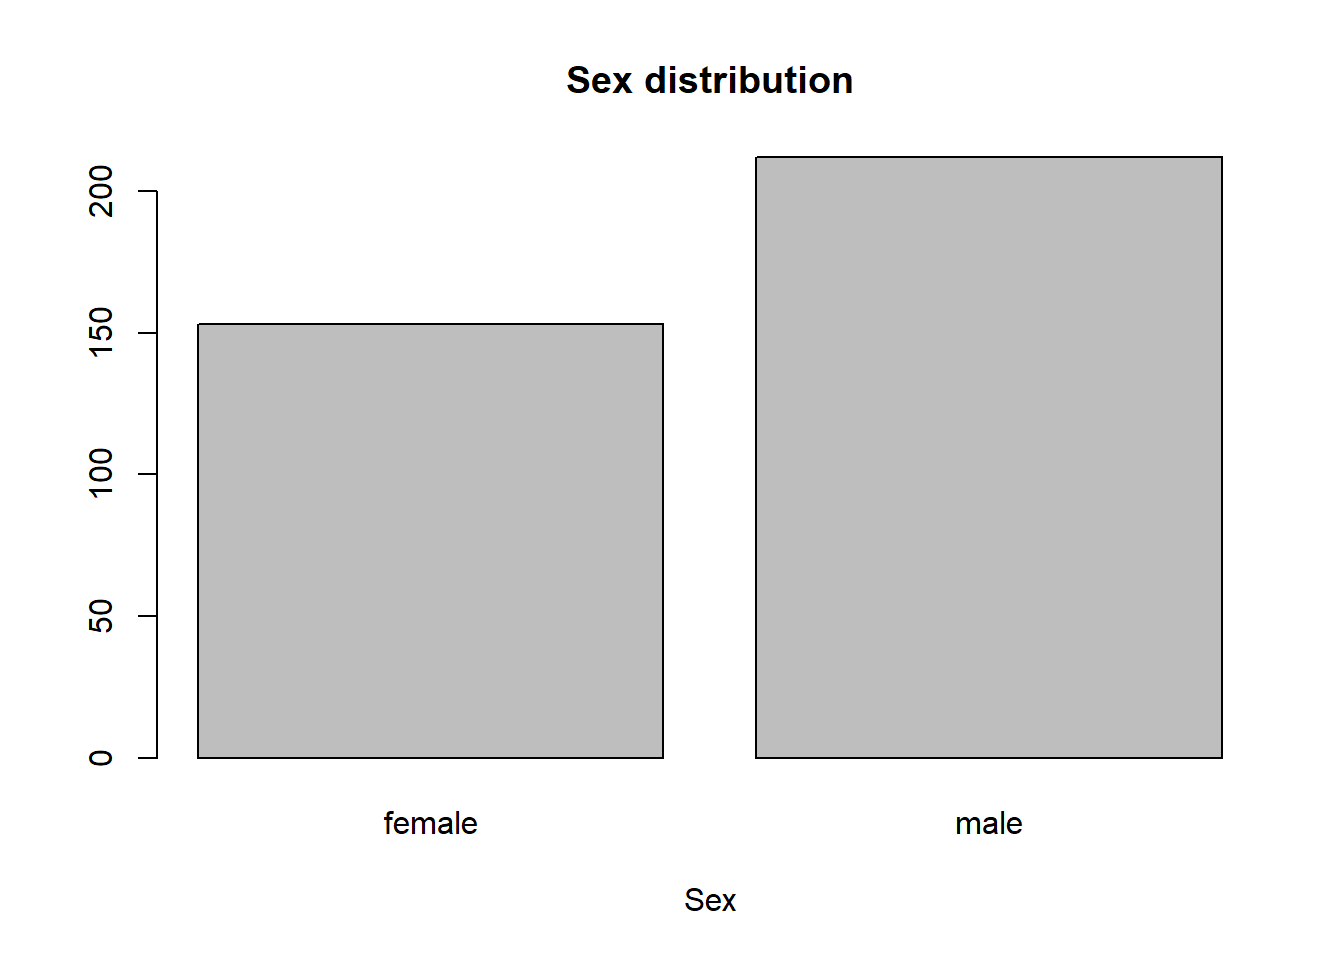
\includegraphics{R_book_KIM_and_Arifin_files/figure-latex/unnamed-chunk-43-1.pdf}

\subsection{One variable: A numerical
variable}\label{one-variable-a-numerical-variable}

histogram

\begin{Shaded}
\begin{Highlighting}[]
\KeywordTok{hist}\NormalTok{(dataSPSS}\OperatorTok{$}\NormalTok{age, }\DataTypeTok{main =} \StringTok{'Age'}\NormalTok{,}
     \DataTypeTok{xlab=}\StringTok{'Age in years'}\NormalTok{,}
     \DataTypeTok{ylab=}\StringTok{'Count'}\NormalTok{)}
\end{Highlighting}
\end{Shaded}

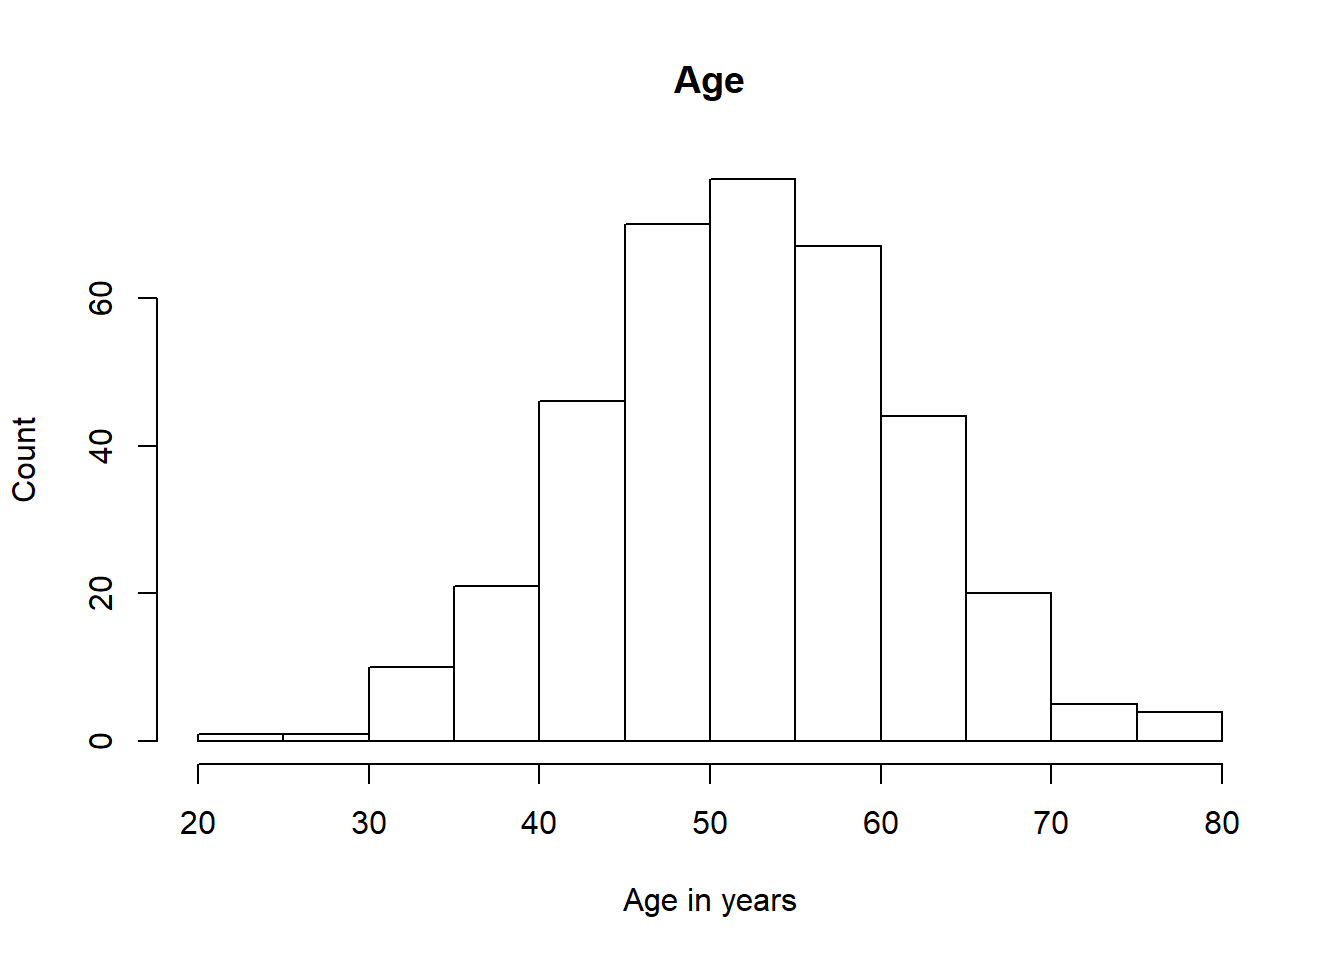
\includegraphics{R_book_KIM_and_Arifin_files/figure-latex/unnamed-chunk-44-1.pdf}

\subsection{Two variables : A numerical with another numerical
variable}\label{two-variables-a-numerical-with-another-numerical-variable}

We will use \emph{scatterplot} to plot

\begin{Shaded}
\begin{Highlighting}[]
\KeywordTok{plot}\NormalTok{(dataSPSS}\OperatorTok{$}\NormalTok{tahundx, dataSPSS}\OperatorTok{$}\NormalTok{age,}
     \DataTypeTok{main =} \StringTok{'Duration having DM VS age'}\NormalTok{,}
     \DataTypeTok{xlab =} \StringTok{'Duration of DM'}\NormalTok{, }\DataTypeTok{ylab =} \StringTok{'Age'}\NormalTok{,}
     \DataTypeTok{pch =} \DecValTok{19}\NormalTok{)}
\end{Highlighting}
\end{Shaded}

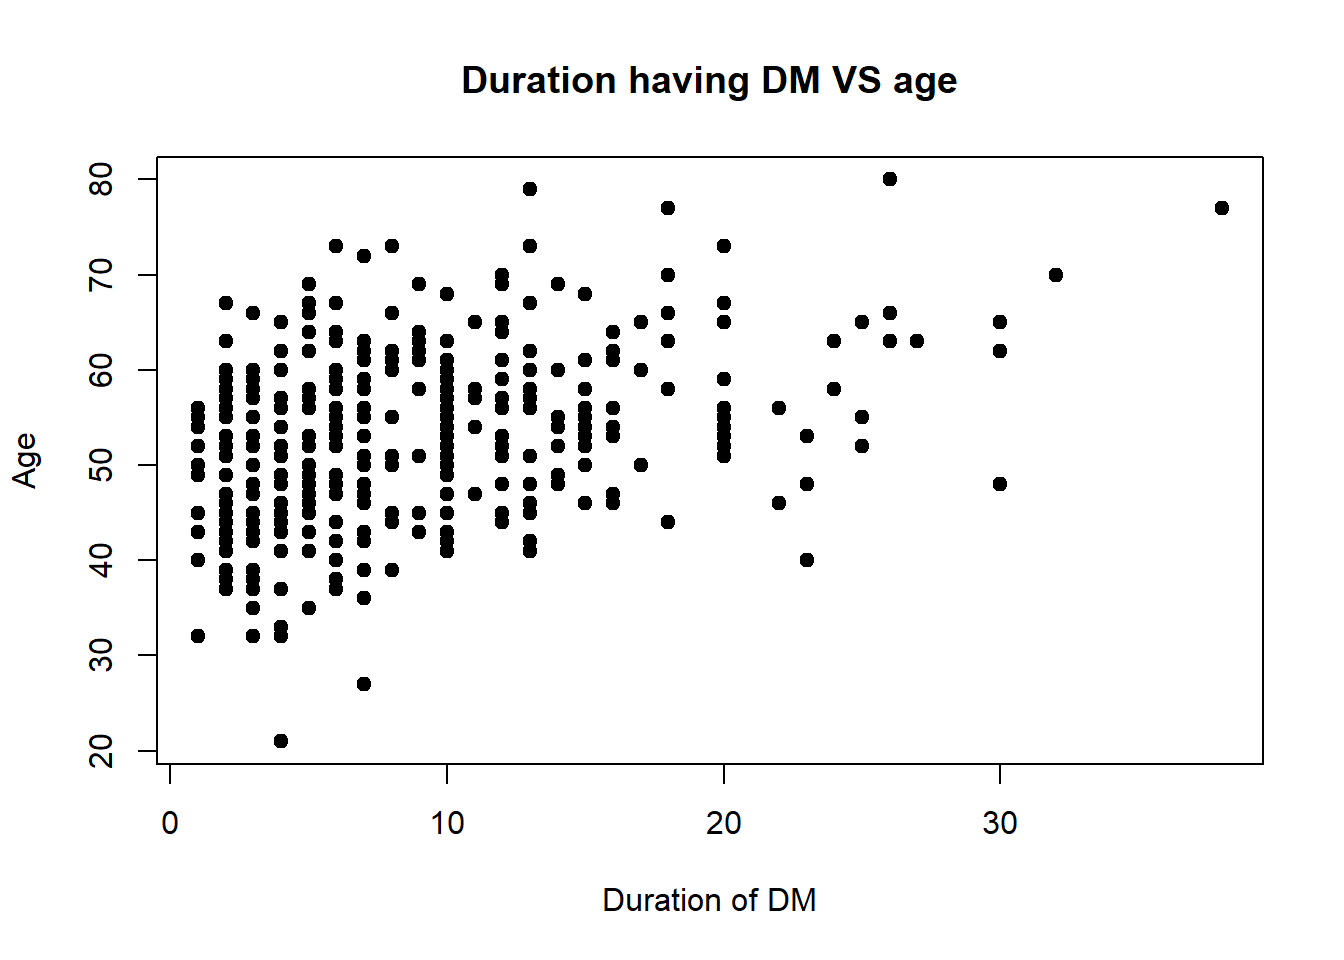
\includegraphics{R_book_KIM_and_Arifin_files/figure-latex/unnamed-chunk-45-1.pdf}

Let us make a fit line

\begin{Shaded}
\begin{Highlighting}[]
\KeywordTok{plot}\NormalTok{(dataSPSS}\OperatorTok{$}\NormalTok{tahundx, dataSPSS}\OperatorTok{$}\NormalTok{age,}
     \DataTypeTok{main =} \StringTok{'Duration having DM VS age'}\NormalTok{,}
     \DataTypeTok{xlab =} \StringTok{'Duration of DM'}\NormalTok{, }\DataTypeTok{ylab =} \StringTok{'Age'}\NormalTok{,}
     \DataTypeTok{pch =} \DecValTok{19}\NormalTok{)}
\KeywordTok{abline}\NormalTok{(}\KeywordTok{lm}\NormalTok{(dataSPSS}\OperatorTok{$}\NormalTok{age}\OperatorTok{~}\NormalTok{dataSPSS}\OperatorTok{$}\NormalTok{tahundx), }\DataTypeTok{col =} \StringTok{'red'}\NormalTok{)}
\end{Highlighting}
\end{Shaded}

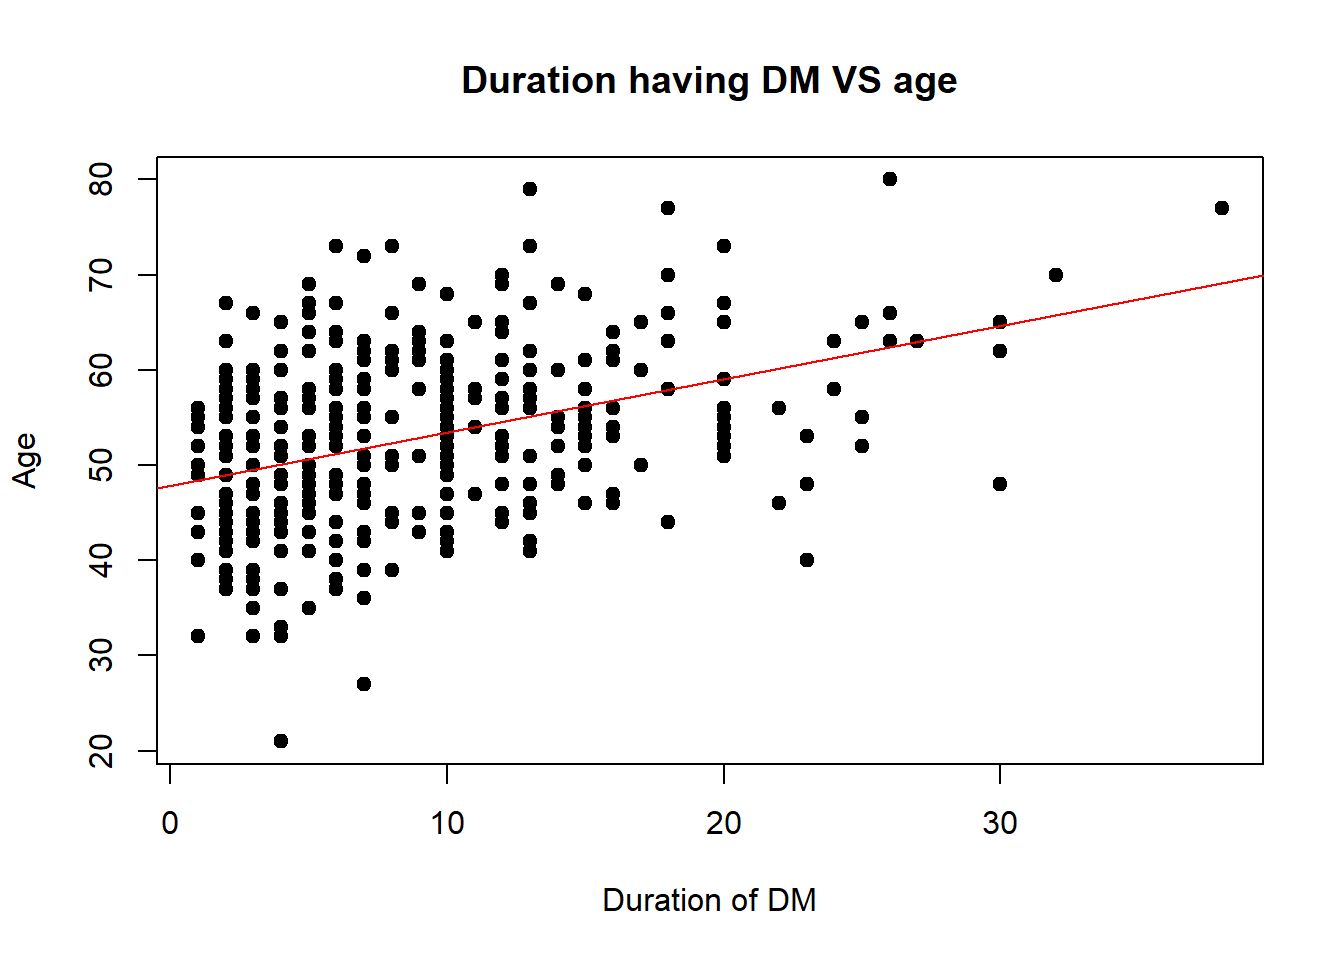
\includegraphics{R_book_KIM_and_Arifin_files/figure-latex/unnamed-chunk-46-1.pdf}

and a lowess

\begin{Shaded}
\begin{Highlighting}[]
\KeywordTok{plot}\NormalTok{(dataSPSS}\OperatorTok{$}\NormalTok{tahundx, dataSPSS}\OperatorTok{$}\NormalTok{age,}
     \DataTypeTok{main =} \StringTok{'Duration having DM VS age'}\NormalTok{,}
     \DataTypeTok{xlab =} \StringTok{'Duration of DM'}\NormalTok{, }\DataTypeTok{ylab =} \StringTok{'Age'}\NormalTok{,}
     \DataTypeTok{pch =} \DecValTok{19}\NormalTok{)}
\KeywordTok{lines}\NormalTok{(}\KeywordTok{lowess}\NormalTok{(dataSPSS}\OperatorTok{$}\NormalTok{tahundx,dataSPSS}\OperatorTok{$}\NormalTok{age), }\DataTypeTok{col =} \StringTok{'blue'}\NormalTok{)}
\end{Highlighting}
\end{Shaded}

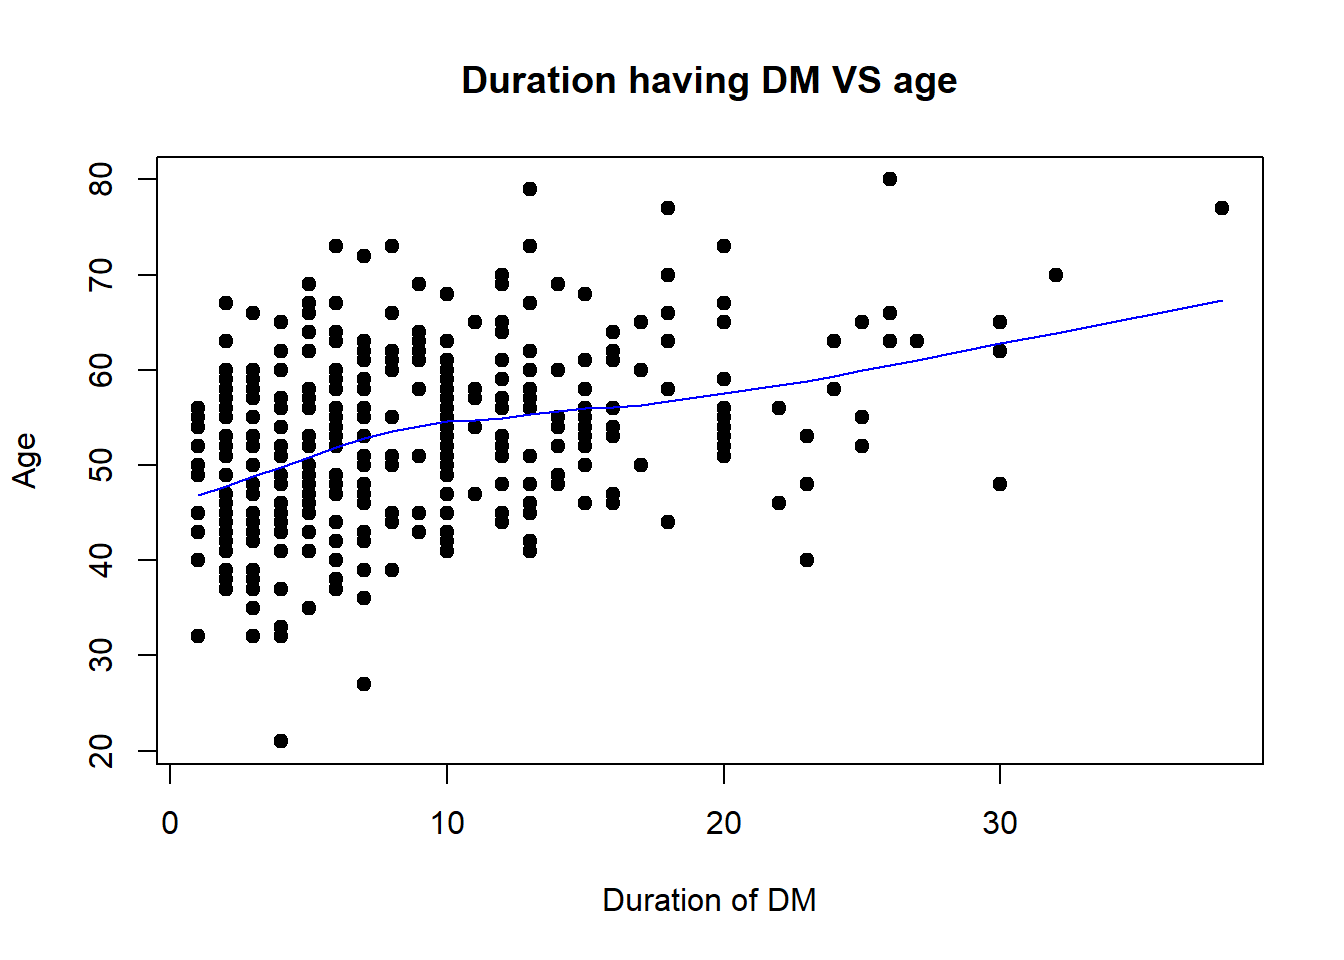
\includegraphics{R_book_KIM_and_Arifin_files/figure-latex/unnamed-chunk-47-1.pdf}

\subsection{Two variables : A categorical variable with a categorical
variable}\label{two-variables-a-categorical-variable-with-a-categorical-variable}

Now, we will plot 2 categorical variables simultenously.

First, we will use stacked barchart

\begin{Shaded}
\begin{Highlighting}[]
\NormalTok{compl.sex<-}\KeywordTok{table}\NormalTok{(dataSPSS}\OperatorTok{$}\NormalTok{complica,dataSPSS}\OperatorTok{$}\NormalTok{sex)}
\NormalTok{compl.sex}
\end{Highlighting}
\end{Shaded}

\begin{verbatim}
##      
##       female male
##   no     105  120
##   yes     48   92
\end{verbatim}

\begin{Shaded}
\begin{Highlighting}[]
\KeywordTok{barplot}\NormalTok{(compl.sex,}
        \DataTypeTok{main=}\StringTok{'Complications by sex'}\NormalTok{,}
        \DataTypeTok{xlab=}\StringTok{'Sex'}\NormalTok{,}
        \DataTypeTok{col=}\KeywordTok{c}\NormalTok{(}\StringTok{'blue'}\NormalTok{,}\StringTok{'red'}\NormalTok{),}
        \DataTypeTok{legend=}\KeywordTok{c}\NormalTok{(}\StringTok{'No'}\NormalTok{,}\StringTok{'Yes'}\NormalTok{))}
\end{Highlighting}
\end{Shaded}

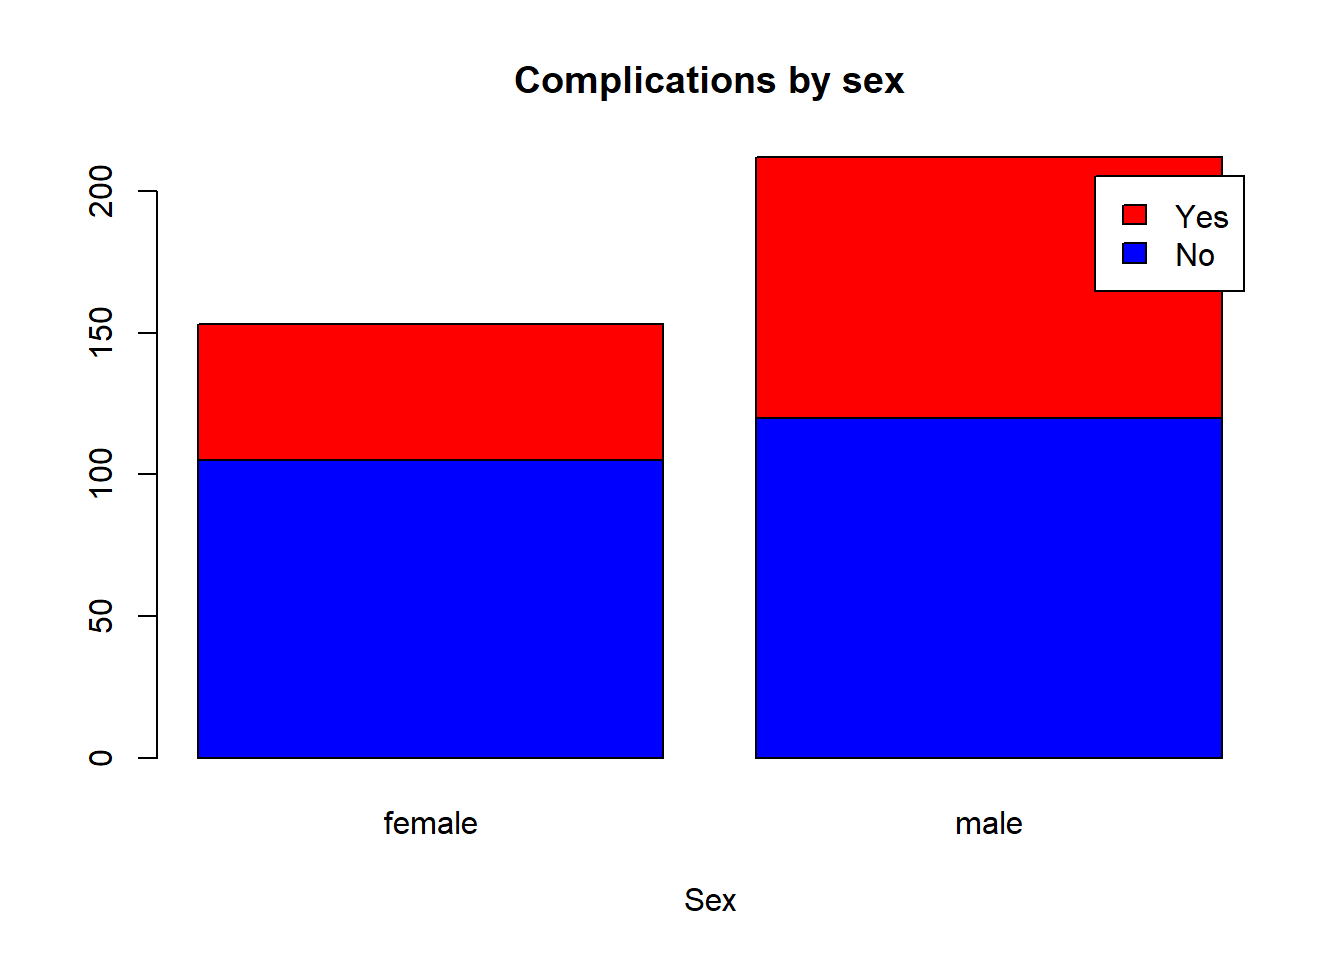
\includegraphics{R_book_KIM_and_Arifin_files/figure-latex/unnamed-chunk-48-1.pdf}

Next, we will use grouped barchart

\begin{Shaded}
\begin{Highlighting}[]
\NormalTok{compl.sex}
\end{Highlighting}
\end{Shaded}

\begin{verbatim}
##      
##       female male
##   no     105  120
##   yes     48   92
\end{verbatim}

\begin{Shaded}
\begin{Highlighting}[]
\KeywordTok{barplot}\NormalTok{(compl.sex,}
        \DataTypeTok{main =} \StringTok{'Complications according to sex'}\NormalTok{,}
        \DataTypeTok{xlab =} \StringTok{'Sex'}\NormalTok{,}
        \DataTypeTok{col =} \KeywordTok{c}\NormalTok{(}\StringTok{'blue'}\NormalTok{,}\StringTok{'red'}\NormalTok{),}
        \DataTypeTok{legend =} \KeywordTok{c}\NormalTok{(}\StringTok{'no'}\NormalTok{,}\StringTok{'yes'}\NormalTok{),}
        \DataTypeTok{beside =} \OtherTok{TRUE}\NormalTok{)}
\end{Highlighting}
\end{Shaded}

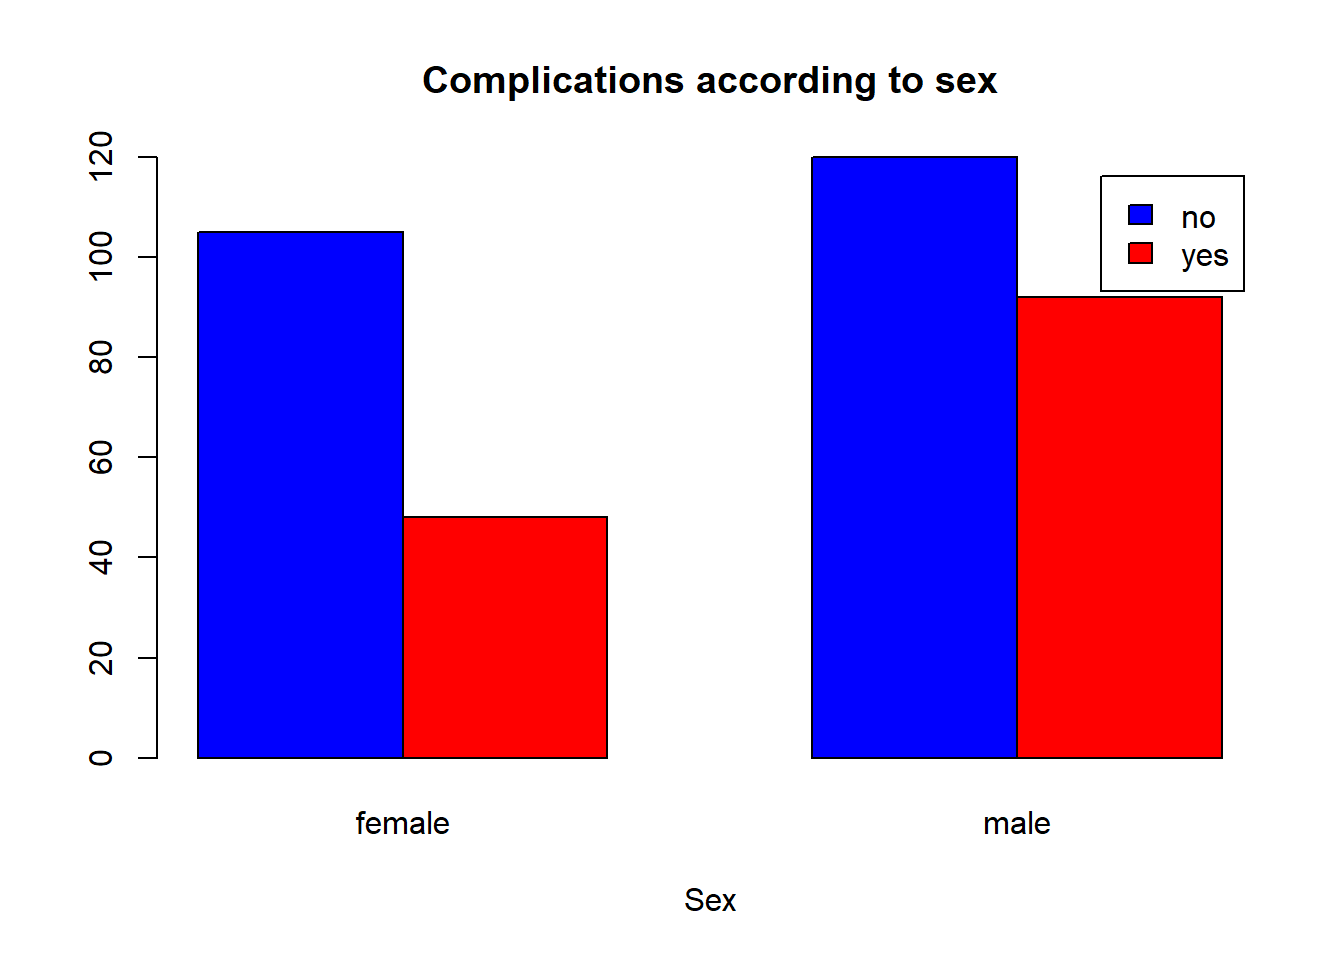
\includegraphics{R_book_KIM_and_Arifin_files/figure-latex/unnamed-chunk-49-1.pdf}

\chapter{Preparing R}\label{preparing-r}

\section{Objectives}\label{objectives}

The objectives of this lecture are:

\begin{enumerate}
\def\labelenumi{\arabic{enumi}.}
\tightlist
\item
  To ensure that the installation of R is correct
\item
  To ensure that the installation of RStudio is correct
\item
  To be able to install R packages
\item
  To be able to create a working directory
\end{enumerate}

\subsection{Installation of R}\label{installation-of-r}

\begin{itemize}
\tightlist
\item
  The latest version of R is R version 3.4.1 (2017-06-30), Single
  Candle.
\item
  R can be installed inside Linux, Mac OS and Windows (of course)
\item
  The installation files (tar.gz, binaries) can be downloaded from
  \url{https://cran.r-project.org/}
\item
  Users can install different versions of R in a same machine or
  computer
\item
  There is no need to uninstall if you want to upgrade currently
  installed R
\end{itemize}

\begin{figure}
\centering
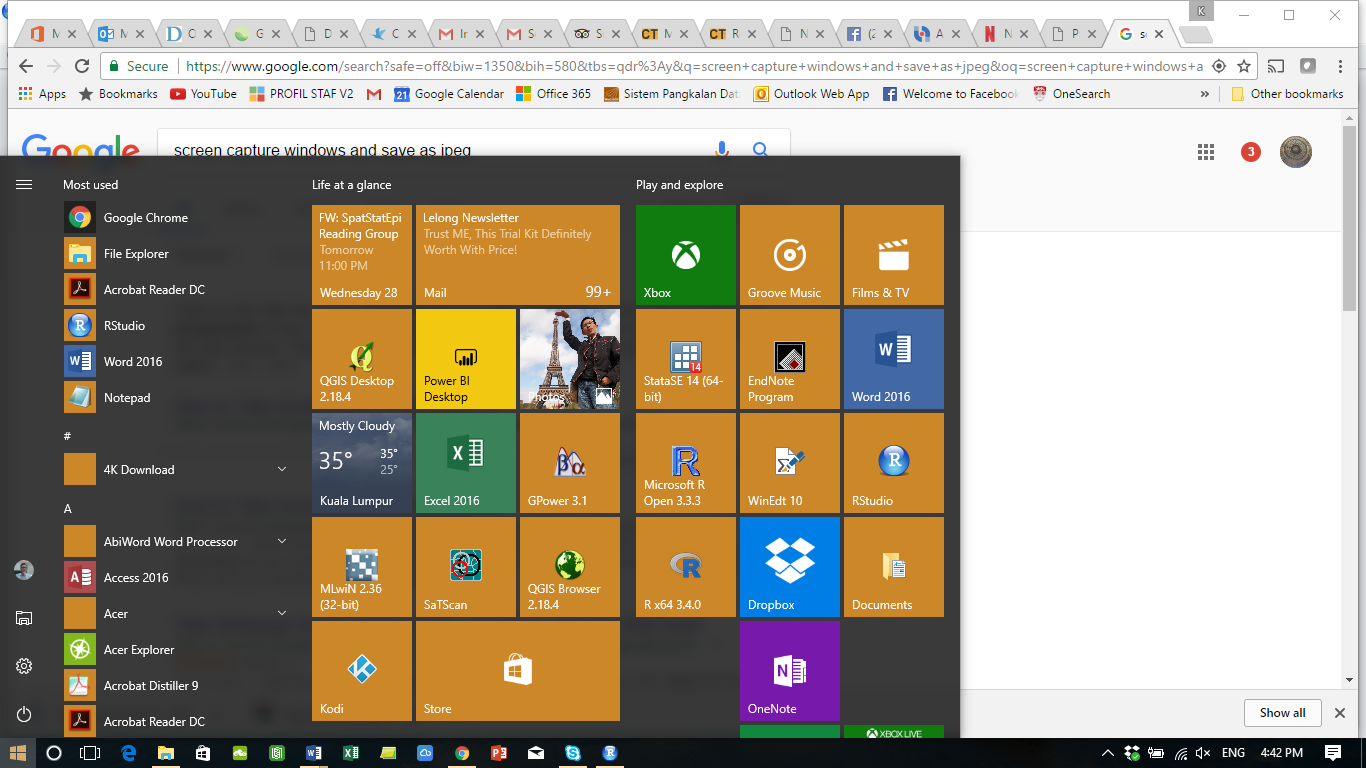
\includegraphics{R.png}
\caption{Succesful R installation}
\end{figure}

\subsubsection{Starting R}\label{starting-r}

Double click on R icon and you should get this

\begin{figure}
\centering
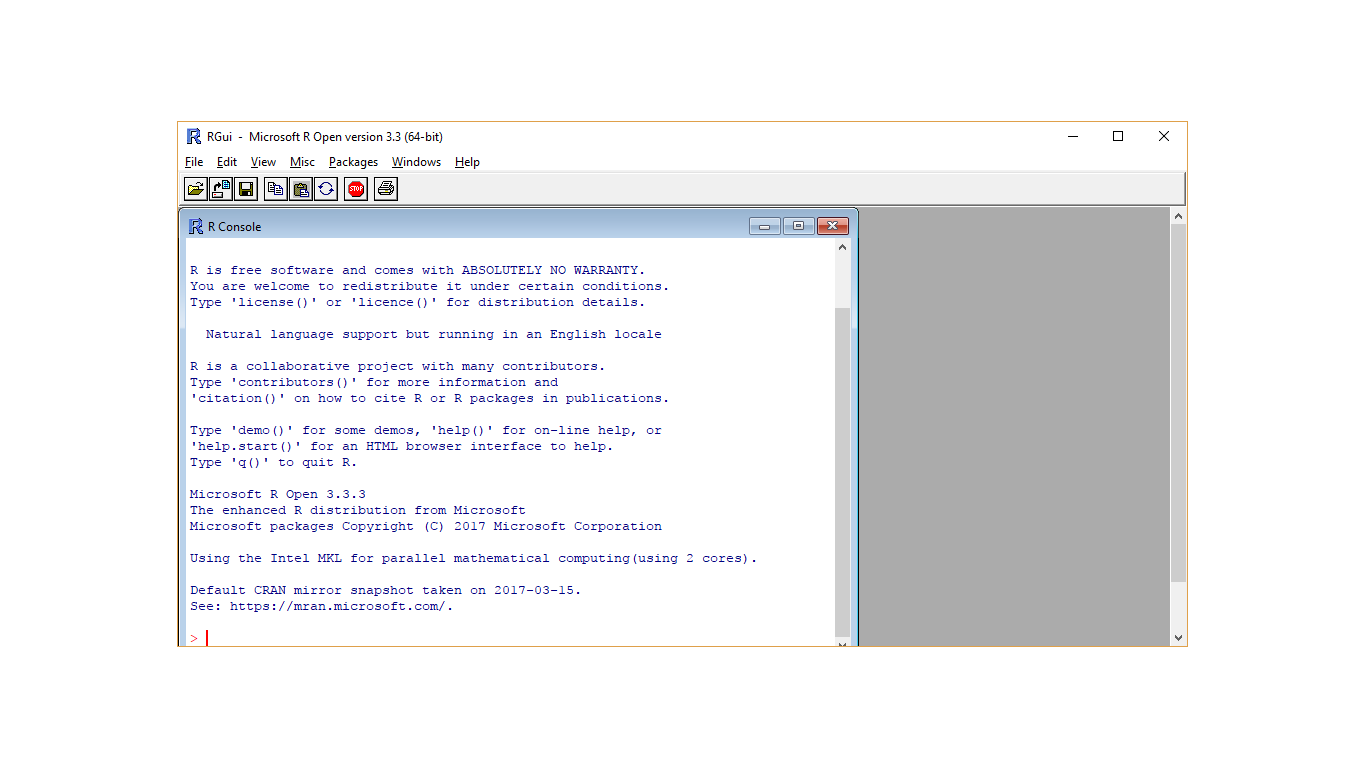
\includegraphics{openr.png}
\caption{R in action}
\end{figure}

\subsection{Installation of RStudio}\label{installation-of-rstudio}

First, make sure you have RStudio successfully installed.

\begin{figure}
\centering
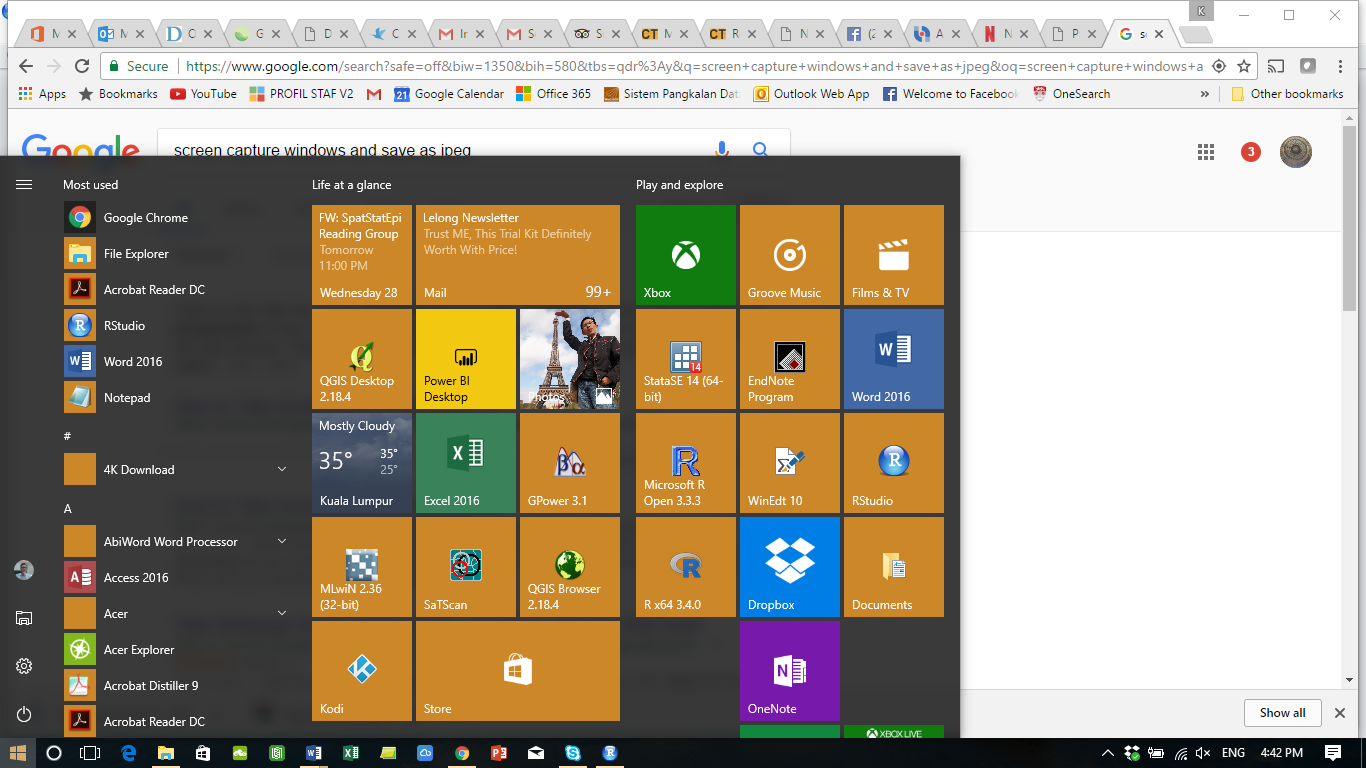
\includegraphics{R.png}
\caption{Succesful RStudio installation}
\end{figure}

\subsubsection{Starting RStudio}\label{starting-rstudio}

You can double click on RStudio icon and you will see this:

\begin{figure}
\centering
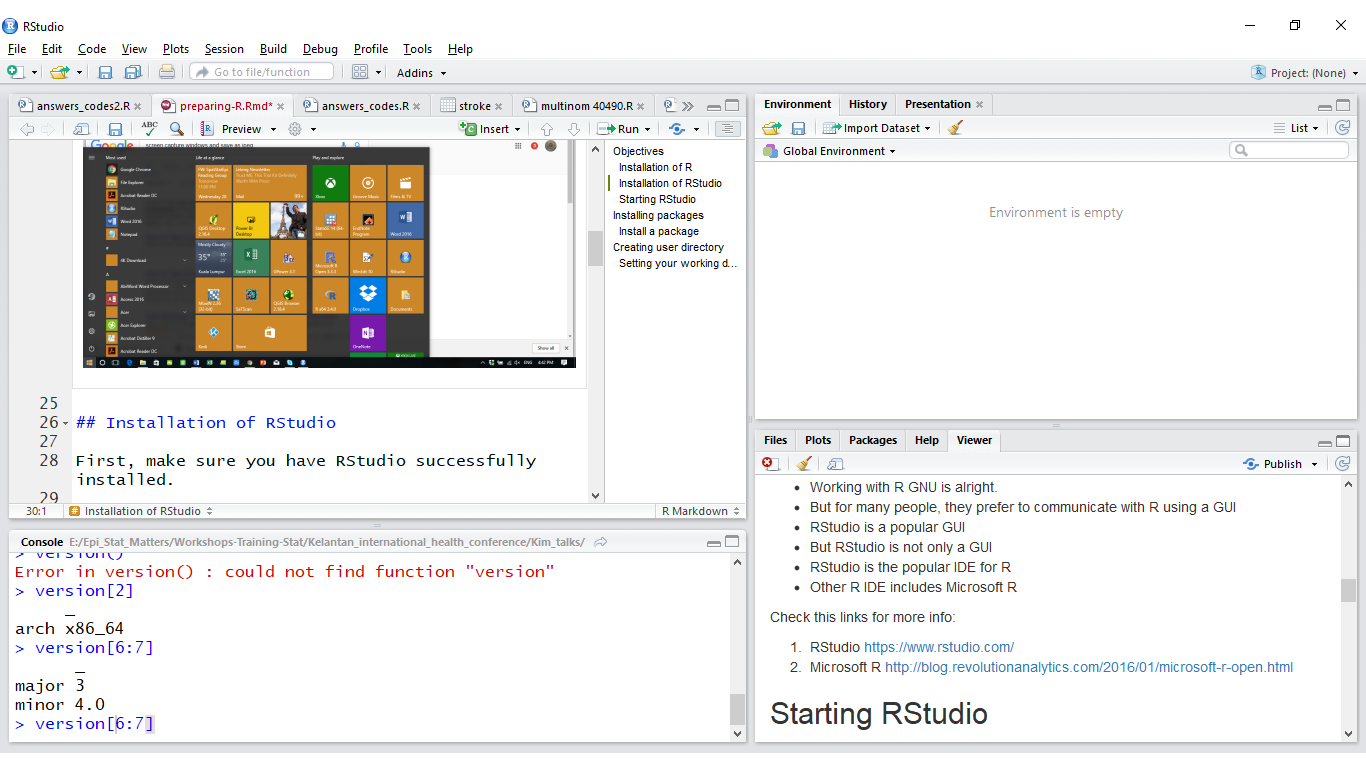
\includegraphics{rstudio.png}
\caption{RStudio sucessfully open}
\end{figure}

\subsubsection{Why RStudio?}\label{why-rstudio}

\begin{itemize}
\tightlist
\item
  Working with R GNU is alright.
\item
  But for many people, they prefer to communicate with R using a GUI
\item
  RStudio is a popular GUI
\item
  But RStudio is not only a GUI
\item
  RStudio is the popular IDE for R
\item
  Other R IDE includes Microsoft R
\end{itemize}

Check this links for more info:

\begin{enumerate}
\def\labelenumi{\arabic{enumi}.}
\tightlist
\item
  RStudio \url{https://www.rstudio.com/}
\item
  Microsoft R
  \url{http://blog.revolutionanalytics.com/2016/01/microsoft-r-open.html}
\end{enumerate}

\subsubsection{RStudio interface}\label{rstudio-interface}

\begin{itemize}
\tightlist
\item
  Depending on your OS, you may start RStudio differently.
\item
  Here we assume you are working with Windows OS
\item
  You should be able to see 4 panes in the layout.
\end{itemize}

\subsubsection{RStudio panes}\label{rstudio-panes}

You should see that - the lower left pane tells you about your R
information (the console pane) - the upper left pane is to show files
that are open - the upper right for the `Environment, History and
Presentation' pane - the lower right pane is for to list file names,
show plots, show packages, display help document and view outputs (such
as html file)

\begin{figure}
\centering
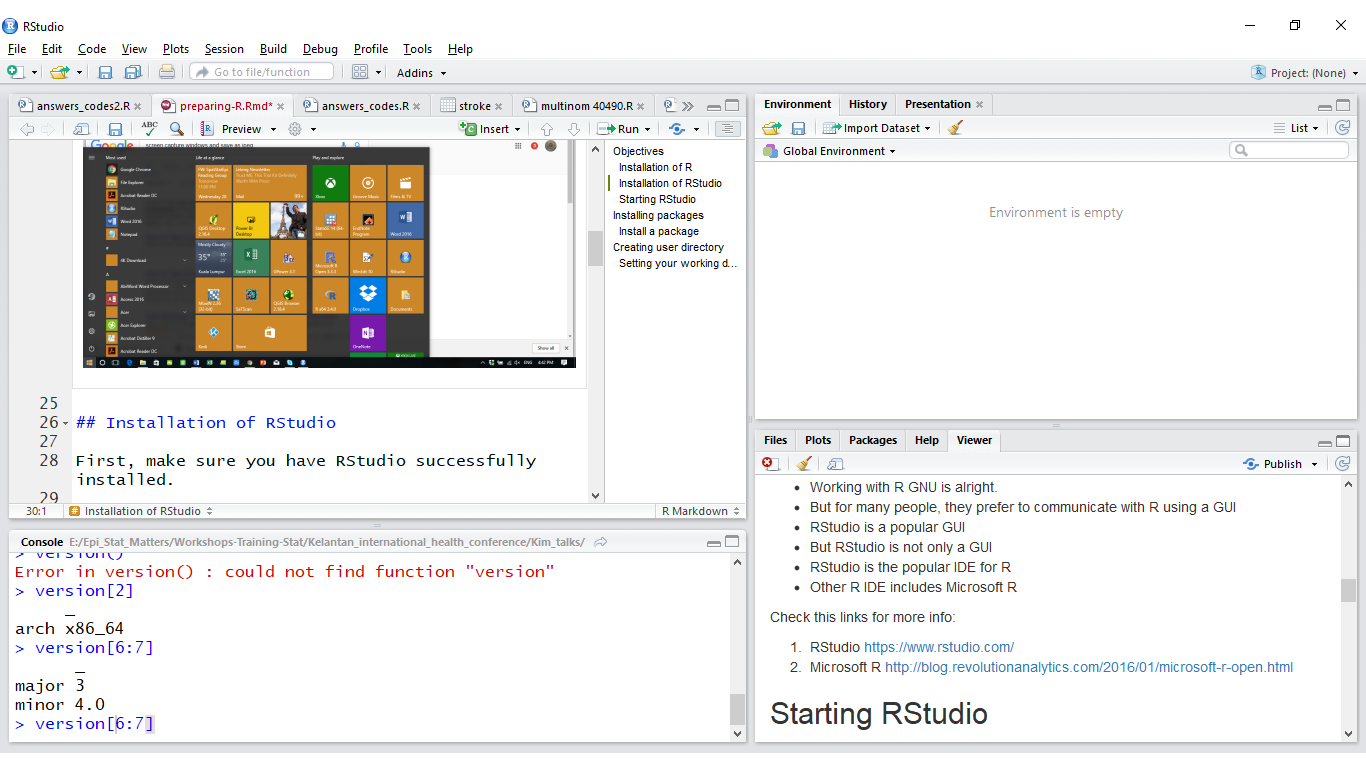
\includegraphics{rstudio.png}
\caption{RStudio sucessfully open}
\end{figure}

\section{Installing packages}\label{installing-packages}

R uses packages to perform its tasks.

There are two common packages:

\begin{enumerate}
\def\labelenumi{\arabic{enumi}.}
\tightlist
\item
  \texttt{base} packages
\item
  \texttt{user-contributed} packages
\end{enumerate}

\begin{itemize}
\tightlist
\item
  The base packages come with the installation of R
\item
  The base package provides basic but adequate functions to perform many
  standard data management, visualization and analysis.
\item
  However, user needs to install user-contributed packages if they need
  to perform functions (tasks) not available in the base package
\item
  User-contributed packages allow users to perform more advanced and
  more complicated functions
\item
  There are more than 10200 packages as of March 2017
\end{itemize}

For a complete list of packages, see
\url{https://cran.r-project.org/web/packages/}

\subsection{Package installation}\label{package-installation}

You can install user-contributed packages through:

\begin{enumerate}
\def\labelenumi{\arabic{enumi}.}
\tightlist
\item
  internet (to cran)
\item
  Github packages
\item
  local zip files
\end{enumerate}

In this session, we will learn to install a few small packages. I have
installed them. For those who have not,

\begin{enumerate}
\def\labelenumi{\arabic{enumi}.}
\tightlist
\item
  put your cursor in the CONSOLE pane
\item
  type the codes below
\end{enumerate}

\begin{Shaded}
\begin{Highlighting}[]
\KeywordTok{install.packages}\NormalTok{(foreign)}
\KeywordTok{install.packages}\NormalTok{(haven)}
\end{Highlighting}
\end{Shaded}

\begin{enumerate}
\def\labelenumi{\arabic{enumi}.}
\setcounter{enumi}{2}
\tightlist
\item
  click ENTER
\end{enumerate}

\section{Workflow}\label{workflow}

We propose that you always have these steps as your workflow when
working with R:

\begin{enumerate}
\def\labelenumi{\arabic{enumi}.}
\tightlist
\item
  Set working directory
\item
  Read data
\item
  Explore + Clean data
\item
  Build Model
\item
  Check Model
\end{enumerate}

\section{Working directory}\label{working-directory}

This is a good practice.

User must create or specify the working directory to work with R.

The working directory:

\begin{enumerate}
\def\labelenumi{\arabic{enumi}.}
\tightlist
\item
  stores all the outputs such as the plots, html files, pdf files
\item
  contains your data
\end{enumerate}

Creating a working directory is a simple BUT an important step.

Unfortunately, many users do not pay attention to this and forget to set
it. So, pay attention so you will not get lost.

\subsection{Creating your working
directory}\label{creating-your-working-directory}

Follow this steps:

\begin{enumerate}
\def\labelenumi{\arabic{enumi}.}
\tightlist
\item
  Make a folder in D directory D:\\
\item
  Name it as \emph{myfolder}
\end{enumerate}

You will see this:

\begin{figure}
\centering
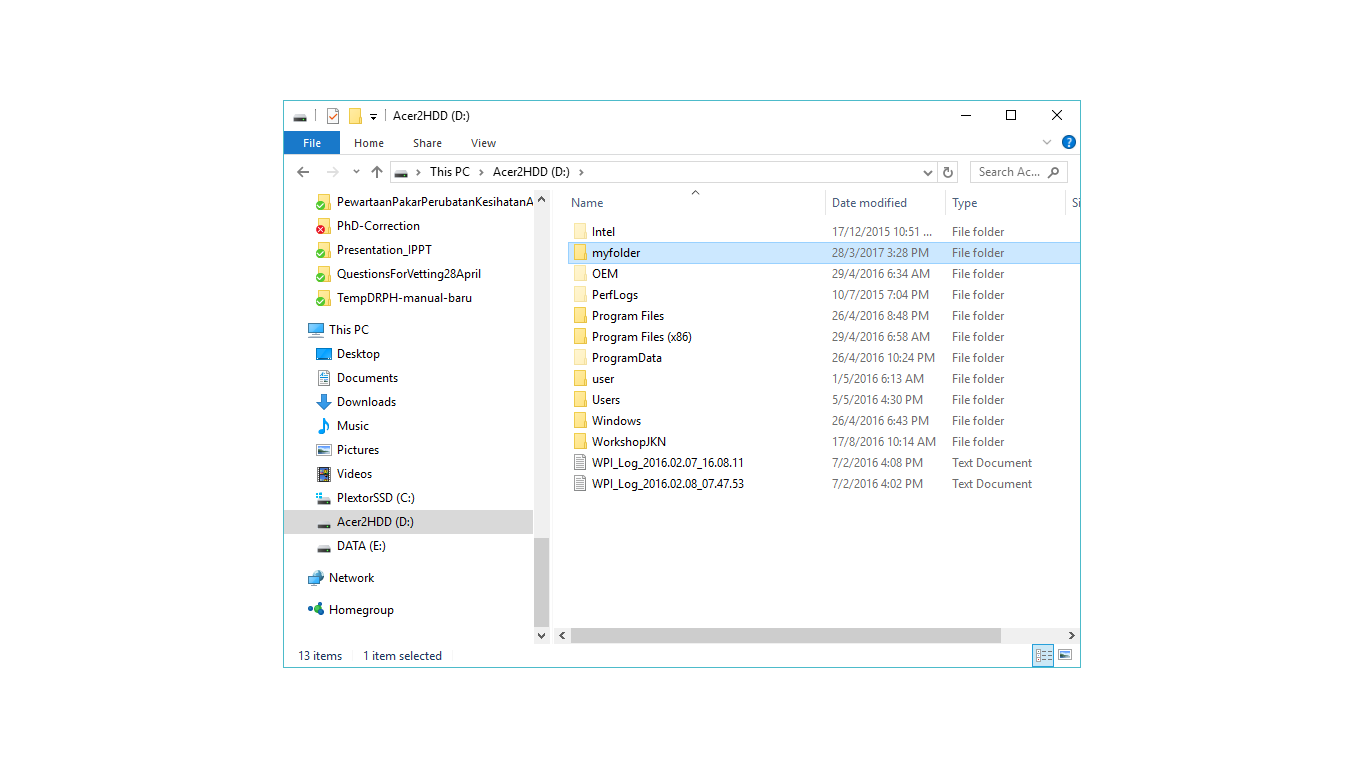
\includegraphics{myfolder.png}
\caption{myfolder}
\end{figure}

\subsection{Setting your working
directory}\label{setting-your-working-directory}

To set your working directory:

\begin{enumerate}
\def\labelenumi{\arabic{enumi}.}
\tightlist
\item
  Go back to RStudio pane
\item
  In the FILE pane, click the \emph{three small dots}
\item
  Navigate to \emph{myfolder}
\item
  Click \emph{More}
\item
  Click \emph{Set as working directory}
\end{enumerate}

\begin{itemize}
\tightlist
\item
  or simply use \emph{setwd} to do so.
\end{itemize}

\begin{Shaded}
\begin{Highlighting}[]
\KeywordTok{setwd}\NormalTok{(}\StringTok{'D:/myfolder'}\NormalTok{)}
\end{Highlighting}
\end{Shaded}

\begin{itemize}
\tightlist
\item
  type \emph{getwd} to confirm
\end{itemize}

\begin{Shaded}
\begin{Highlighting}[]
\KeywordTok{getwd}\NormalTok{()}
\end{Highlighting}
\end{Shaded}

\begin{verbatim}
## [1] "E:/R_book"
\end{verbatim}

\chapter{Reading statistical data}\label{reading-statistical-data}

\section{Objectives}\label{objectives-1}

At the end of the lecture, participants are:

\begin{enumerate}
\def\labelenumi{\arabic{enumi}.}
\tightlist
\item
  able to read various data formats into R
\item
  able to export data from R into various data format
\item
  able to create R-markdown document
\end{enumerate}

\section{Data formats}\label{data-formats}

R can read datasets from different formats.

The \texttt{base} package enables us to read \texttt{.txt} and
\texttt{.csv} files.

You can also use the point and click method to read data. Go to File
-\textgreater{} Import Dataset -\textgreater{} From \ldots{}

To read datasets from SPSS (\texttt{.sav}), Stata (\texttt{.dta}), Excel
(\texttt{xlsx}) and SAS, we need to load special packages.

There are more than 1 packages you can use to read and write data
from/to different spreadsheet or statistical software.

The packages include:

\begin{enumerate}
\def\labelenumi{\arabic{enumi}.}
\tightlist
\item
  \texttt{haven}
\item
  \texttt{foreign}
\item
  \texttt{readxl}
\item
  \texttt{readr}
\end{enumerate}

\section{Reading data into R}\label{reading-data-into-r}

\subsection{Reading csv file}\label{reading-csv-file}

Let us read a \texttt{.csv} files names as \texttt{metab.csv}.

We would like to create an object named as \texttt{met\_data} to
represent the read \texttt{metab.csv}. We can do this:

\begin{Shaded}
\begin{Highlighting}[]
\NormalTok{met_data <-}\StringTok{ }\KeywordTok{read.csv}\NormalTok{(}\StringTok{'metab1.csv'}\NormalTok{, }\DataTypeTok{header =} \OtherTok{TRUE}\NormalTok{)}
\end{Highlighting}
\end{Shaded}

header = TRUE means that you will read the first row as the variable
names.

After you have done this, you will see a new object named as
\texttt{met\_data} inside the \emph{environment} pane.

\subsection{Reading dataset from MS Excel
file}\label{reading-dataset-from-ms-excel-file}

You can read dataset from Excel using 2 methods

\begin{enumerate}
\def\labelenumi{\arabic{enumi}.}
\tightlist
\item
  point and click method. File - Import Dataset - from Excel
\item
  \texttt{readxl} package
\end{enumerate}

To read data using specific packages such as \texttt{readxl} package:

\begin{enumerate}
\def\labelenumi{\arabic{enumi}.}
\tightlist
\item
  you need to install the library first using
  \texttt{install.packages()}
\item
  After that, load the library using \texttt{library(readxl)}
\item
  Type \texttt{read\_excel()} with relevant arguments to read the data
  into RStudio
\end{enumerate}

\begin{Shaded}
\begin{Highlighting}[]
\KeywordTok{library}\NormalTok{(readxl)}
\NormalTok{dataexcel <-}\StringTok{ }\KeywordTok{read_excel}\NormalTok{(}\StringTok{'eye.xlsx'}\NormalTok{, }\DataTypeTok{sheet =} \DecValTok{1}\NormalTok{)}
\end{Highlighting}
\end{Shaded}

The example above means that we read an MS Excel file named as
\texttt{eye.xlsx} and named it as \texttt{dataexcel}.

\subsection{Reading dataset from SPSS file
(.sav)}\label{reading-dataset-from-spss-file-.sav-1}

Dataset in SPSS format will end with \texttt{.sav}.

To read SPSS data into R we may use \texttt{foreign} or \texttt{haven}
packages.

After reading the \texttt{.sav} file, an object will be created based on
what we named it.

The example below shows that an object named as
\texttt{dataSPSS}represents the SPSS data \texttt{cholest.sav}that we
just read into RStudio.

\begin{Shaded}
\begin{Highlighting}[]
\KeywordTok{library}\NormalTok{(foreign)}
\NormalTok{dataSPSS <-}\StringTok{ }\KeywordTok{read.spss}\NormalTok{(}\StringTok{'cholest.sav'}\NormalTok{, }\DataTypeTok{to.data.frame =} \OtherTok{TRUE}\NormalTok{)}
\end{Highlighting}
\end{Shaded}

\begin{verbatim}
## re-encoding from UTF-8
\end{verbatim}

\subsection{Reading dataset from Stata
(.dta)}\label{reading-dataset-from-stata-.dta}

Dataset in Stata format will end with \texttt{.dta}.

To read Stata data into R we may use \texttt{foreign} or \texttt{haven}
packages.

After reading the \texttt{.dta} file, similarly an object will be
created - in this case, we named it as \texttt{dataSTATA}.

\texttt{dataSTATA} is an object that represents the Stata data (now in
the memory) that we just read \texttt{metab1.dta}into RStudio.

\begin{Shaded}
\begin{Highlighting}[]
\NormalTok{datastata <-}\StringTok{ }\KeywordTok{read.dta}\NormalTok{(}\StringTok{'metab1.dta'}\NormalTok{, }\DataTypeTok{convert.factors =} \OtherTok{TRUE}\NormalTok{)}
\end{Highlighting}
\end{Shaded}

\subsection{Alternative methods or
package}\label{alternative-methods-or-package}

\begin{enumerate}
\def\labelenumi{\arabic{enumi}.}
\tightlist
\item
  You can go to File - Read Datasets
\item
  You may use \textbf{haven} package to read SAS, SPSS and Stata file.
\end{enumerate}

\begin{Shaded}
\begin{Highlighting}[]
\KeywordTok{library}\NormalTok{(haven)}
\NormalTok{dataSPSS2 <-}\StringTok{ }\KeywordTok{read_sav}\NormalTok{(}\StringTok{'cholest.sav'}\NormalTok{)}
\NormalTok{dataSTATA2 <-}\StringTok{ }\KeywordTok{read_dta}\NormalTok{(}\StringTok{'cholest.dta'}\NormalTok{)}
\end{Highlighting}
\end{Shaded}

\subsection{Other data format}\label{other-data-format}

Other important data formats that might be useful in epidemiology and
statistics are:

\begin{enumerate}
\def\labelenumi{\arabic{enumi}.}
\tightlist
\item
  shapefile \texttt{.shp}
\item
  text file \texttt{.txt}
\item
  text file \texttt{.dat}
\item
  \texttt{XML} file
\item
  images file \texttt{DICOM}
\end{enumerate}

We will not cover these today.

\section{Exporting data from R}\label{exporting-data-from-r}

You can also export data into various formats using similar packages.

For example,

\begin{enumerate}
\def\labelenumi{\arabic{enumi}.}
\tightlist
\item
  to export data into a \emph{comma separated version} (.csv) file, we
  can use \texttt{write.csv} function.
\item
  to export data into stata format, we can use \texttt{write.dta}
  function
\end{enumerate}

\begin{Shaded}
\begin{Highlighting}[]
\NormalTok{export_csv <-}\StringTok{ }\KeywordTok{write.csv}\NormalTok{(dataSPSS, }\StringTok{'export_csv.csv'}\NormalTok{)}
\NormalTok{export_stata <-}\StringTok{ }\KeywordTok{write.dta}\NormalTok{(dataexcel, }\StringTok{'export_stata.dta'}\NormalTok{) }
\end{Highlighting}
\end{Shaded}

\chapter{GLM}\label{glm}

\subsection{Objectives}\label{objectives-2}

At the end of the lecture, participants are

\begin{enumerate}
\def\labelenumi{\arabic{enumi}.}
\tightlist
\item
  able to perform linear regression
\item
  able to perform logistic regression
\item
  able to perform Cox proportional hazard regression
\end{enumerate}

\section{Set working directory}\label{set-working-directory}

Set your working directory.

This is a folder that contains your dataset and objects created by R.

\section{Read data}\label{read-data-1}

We will read a stata data into R. This file will read using
\textbf{foreign} package.

We will name the object as \textbf{data1} as an object that represent
the dataset.

This object is a \texttt{data.frame} object

The \textbf{data1} object will remain in the memory unless you close
your RStudio.

\begin{Shaded}
\begin{Highlighting}[]
\KeywordTok{library}\NormalTok{(foreign)}
\NormalTok{data1 <-}\StringTok{ }\KeywordTok{read.dta}\NormalTok{(}\StringTok{'metab1.dta'}\NormalTok{, }\DataTypeTok{convert.factors =} \OtherTok{TRUE}\NormalTok{) }
\KeywordTok{head}\NormalTok{(data1)}
\end{Highlighting}
\end{Shaded}

\begin{verbatim}
##   id2 age sex race marital dm  bmi2 waist hip hba1c  fbs totchol   msbp
## 1   1  42   2    1       1  0 21.31    72  89   5.0 5.41    4.80 113.25
## 2   2  63   2    1       3  1 36.00   125  95   7.2 8.39    8.09 209.00
## 3   3  54   2    1       1  0 37.17   100 118   5.6 5.46    4.32 160.00
## 4   4  46   1    1       1  0 27.34    89  97   5.3 5.82    5.27 134.25
## 5   5  40   2    1       1  0 26.94    79  99   4.8 4.67    6.38 100.00
## 6   6  43   1    1       1  0 28.82   101 112   5.1 4.82    7.48 159.00
##     mdbp gender crural racecat       whr
## 1  73.50 female      0       0 0.8089887
## 2  94.00 female      1       0 1.3157895
## 3  76.75 female      0       0 0.8474576
## 4  87.75   male      1       0 0.9175258
## 5  65.00 female      1       0 0.7979798
## 6 104.00   male      0       0 0.9017857
\end{verbatim}

We use \texttt{head()} function to list the first 6 observations in the
dataset.

\section{Explore and clean data}\label{explore-and-clean-data}

Next we will describe the data and visualize

\begin{enumerate}
\def\labelenumi{\arabic{enumi}.}
\tightlist
\item
  Descriptive
\item
  Visualization
\end{enumerate}

\subsection{Descriptive analysis}\label{descriptive-analysis}

We will check basic descriptive statistics from our data

\begin{Shaded}
\begin{Highlighting}[]
\KeywordTok{library}\NormalTok{(psych)}
\KeywordTok{describe}\NormalTok{(data1)}
\end{Highlighting}
\end{Shaded}

\begin{verbatim}
##         vars   n   mean     sd median trimmed    mad   min    max  range
## id2        1 500 250.50 144.48 250.50  250.50 185.32  1.00 500.00 499.00
## age        2 500  49.04  14.09  48.50   49.06  14.08 18.00  84.00  66.00
## sex        3 500   1.58   0.49   2.00    1.60   0.00  1.00   2.00   1.00
## race       4 500   1.46   0.99   1.00    1.21   0.00  1.00   5.00   4.00
## marital    5 498   1.29   0.65   1.00    1.12   0.00  1.00   3.00   2.00
## dm         6 500   0.11   0.31   0.00    0.01   0.00  0.00   1.00   1.00
## bmi2       7 500  26.28   5.33  25.71   25.95   4.81 14.30  56.08  41.78
## waist      8 500  86.40  12.79  86.00   86.08  11.86 52.00 154.50 102.50
## hip        9 500  98.54  10.75  98.00   98.31  10.38 62.00 153.50  91.50
## hba1c     10 496   5.86   1.47   5.40    5.56   0.44  0.20  13.20  13.00
## fbs       11 486   5.94   2.30   5.39    5.54   1.14  2.59  21.11  18.52
## totchol   12 496   5.83   1.29   5.80    5.76   1.20  2.47  12.29   9.82
## msbp      13 500 134.72  22.77 132.00  132.92  21.68 82.50 225.00 142.50
## mdbp      14 500  80.03  11.51  79.50   79.86  11.49 45.00 120.00  75.00
## gender*   15 500   1.42   0.49   1.00    1.40   0.00  1.00   2.00   1.00
## crural    16 500   0.51   0.50   1.00    0.51   0.00  0.00   1.00   1.00
## racecat   17 500   0.45   0.94   0.00    0.21   0.00  0.00   3.00   3.00
## whr       18 500   0.88   0.11   0.86    0.87   0.08  0.65   1.42   0.77
##          skew kurtosis   se
## id2      0.00    -1.21 6.46
## age      0.01    -0.46 0.63
## sex     -0.31    -1.90 0.02
## race     2.00     2.77 0.04
## marital  1.98     2.28 0.03
## dm       2.52     4.35 0.01
## bmi2     0.97     2.50 0.24
## waist    0.61     2.03 0.57
## hip      0.46     2.21 0.48
## hba1c    2.49     7.80 0.07
## fbs      2.88    11.33 0.10
## totchol  0.73     1.74 0.06
## msbp     0.80     0.68 1.02
## mdbp     0.18    -0.05 0.51
## gender*  0.31    -1.90 0.02
## crural  -0.03    -2.00 0.02
## racecat  1.85     1.87 0.04
## whr      1.72     5.09 0.00
\end{verbatim}

\subsection{Visualization}\label{visualization}

We do not have time to cover for data vizualition.

But for here we would do

\begin{enumerate}
\def\labelenumi{\arabic{enumi}.}
\tightlist
\item
  histogram
\item
  bar charts
\item
  box-plots
\item
  scatterplots
\end{enumerate}

To examine the distribution of our data.

Briefly:

\begin{Shaded}
\begin{Highlighting}[]
\KeywordTok{hist}\NormalTok{(data1}\OperatorTok{$}\NormalTok{age)}
\end{Highlighting}
\end{Shaded}

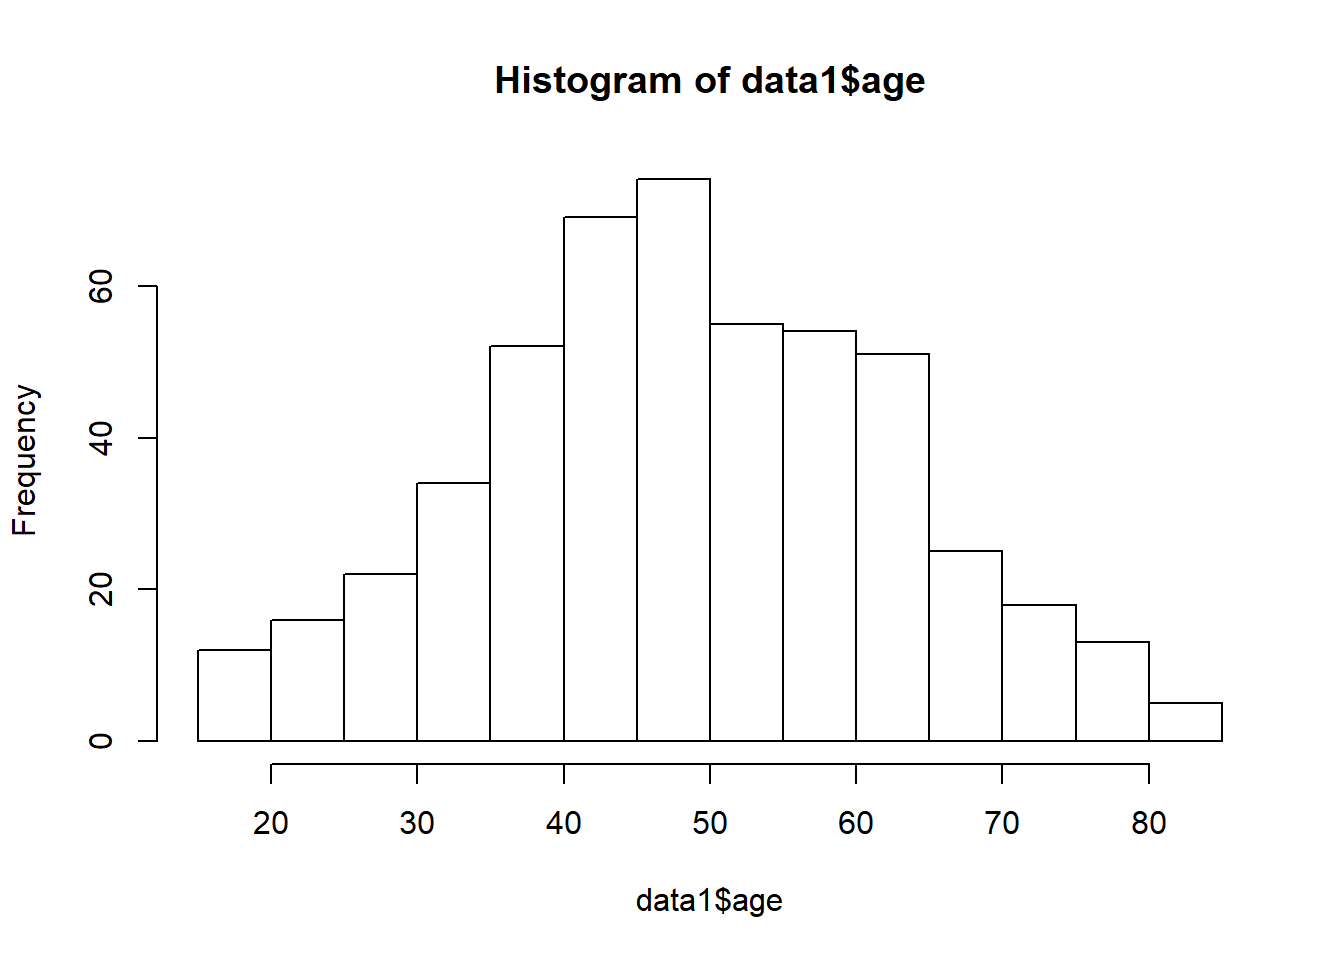
\includegraphics{R_book_KIM_and_Arifin_files/figure-latex/unnamed-chunk-61-1.pdf}

\begin{Shaded}
\begin{Highlighting}[]
\NormalTok{cts_sex <-}\StringTok{ }\KeywordTok{table}\NormalTok{(data1}\OperatorTok{$}\NormalTok{sex)}
\KeywordTok{barplot}\NormalTok{(cts_sex, }\DataTypeTok{names.arg =} \KeywordTok{c}\NormalTok{(}\StringTok{'male'}\NormalTok{,}\StringTok{'female'}\NormalTok{))}
\end{Highlighting}
\end{Shaded}

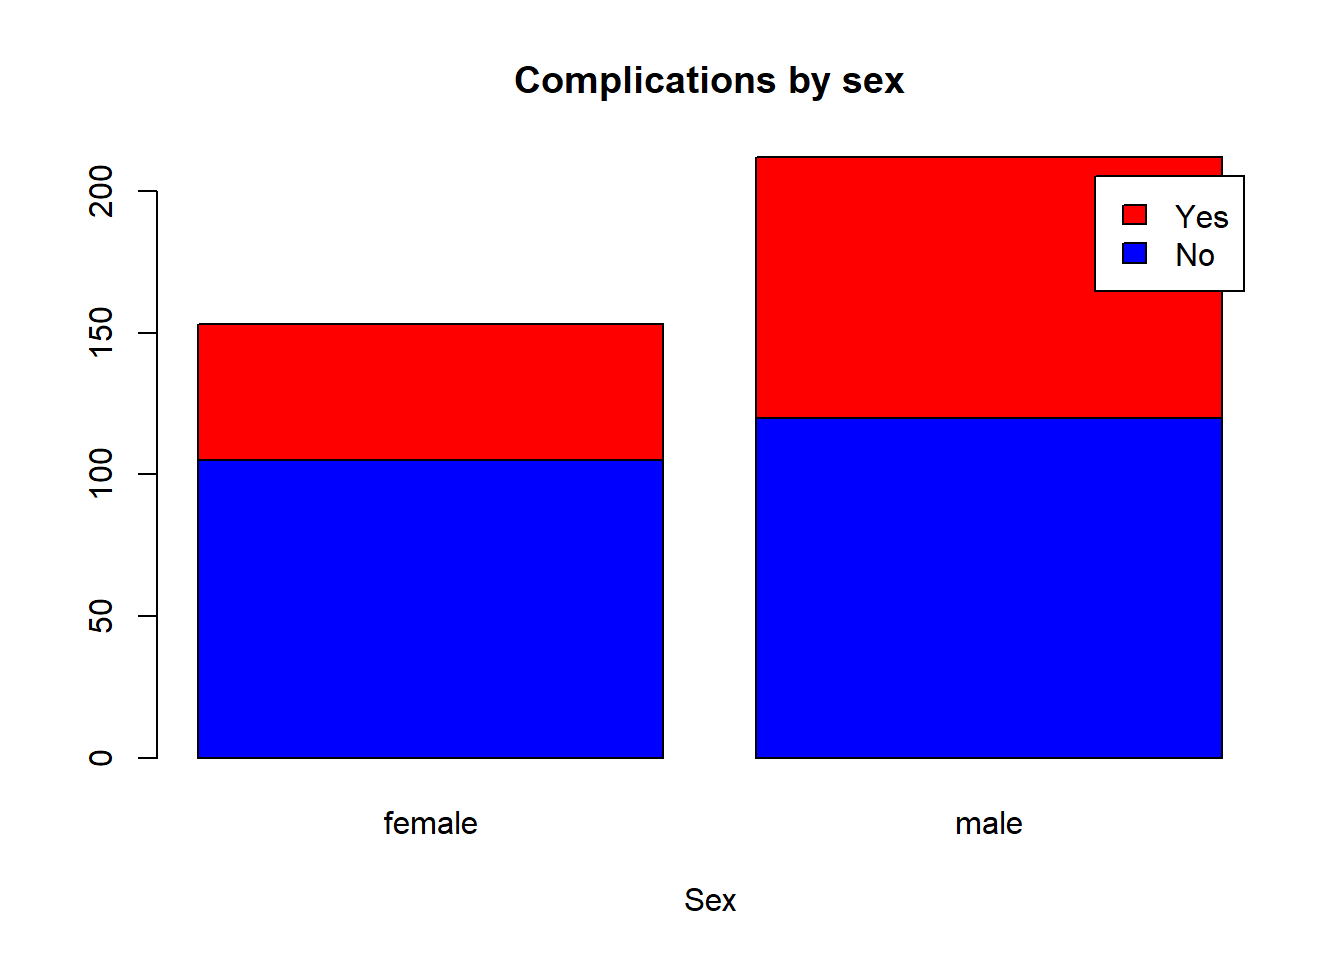
\includegraphics{R_book_KIM_and_Arifin_files/figure-latex/unnamed-chunk-62-1.pdf}

\begin{Shaded}
\begin{Highlighting}[]
\KeywordTok{cor}\NormalTok{(data1[,}\KeywordTok{c}\NormalTok{(}\DecValTok{2}\NormalTok{,}\DecValTok{7}\OperatorTok{:}\DecValTok{14}\NormalTok{ )], }\DataTypeTok{use =} \StringTok{'complete.obs'}\NormalTok{)}
\end{Highlighting}
\end{Shaded}

\begin{verbatim}
##                  age       bmi2      waist          hip     hba1c
## age     1.0000000000 0.01333764 0.20366927 0.0007456519 0.1637614
## bmi2    0.0133376398 1.00000000 0.76631090 0.8333520043 0.1894581
## waist   0.2036692689 0.76631090 1.00000000 0.6481527376 0.2607116
## hip     0.0007456519 0.83335200 0.64815274 1.0000000000 0.1393534
## hba1c   0.1637613510 0.18945815 0.26071159 0.1393533901 1.0000000
## fbs     0.0744876967 0.14530370 0.16664931 0.1081298717 0.6201932
## totchol 0.1680643316 0.03611592 0.07409306 0.0314817073 0.1919677
## msbp    0.4973145998 0.29310141 0.34845937 0.2088822226 0.1012963
## mdbp    0.2395562888 0.39672237 0.38554987 0.3421091043 0.1149683
##               fbs    totchol      msbp       mdbp
## age     0.0744877 0.16806433 0.4973146 0.23955629
## bmi2    0.1453037 0.03611592 0.2931014 0.39672237
## waist   0.1666493 0.07409306 0.3484594 0.38554987
## hip     0.1081299 0.03148171 0.2088822 0.34210910
## hba1c   0.6201932 0.19196773 0.1012963 0.11496827
## fbs     1.0000000 0.23526402 0.0976063 0.11685121
## totchol 0.2352640 1.00000000 0.1286784 0.09181019
## msbp    0.0976063 0.12867845 1.0000000 0.69994756
## mdbp    0.1168512 0.09181019 0.6999476 1.00000000
\end{verbatim}

\section{Linear regression}\label{linear-regression}

We perform linear regression when we assume that distribution of the
outcome variables is normally distributed as a function of certain
covariates (independent variables)

\subsection{Estimation}\label{estimation}

To perform the estimation for linear regression, we can use
\texttt{lm()} function.

Let us model body mass index \emph{bmi} as a function of hip
circumference, mean systolic blood pressure \emph{msbp}, mean diastolic
blood pressure \emph{mdbp} and \emph{gender}

\begin{Shaded}
\begin{Highlighting}[]
\NormalTok{modl <-}\StringTok{ }\KeywordTok{lm}\NormalTok{(bmi2 }\OperatorTok{~}\StringTok{ }\NormalTok{hip }\OperatorTok{+}\StringTok{ }\NormalTok{msbp }\OperatorTok{+}\StringTok{ }\NormalTok{mdbp }
           \OperatorTok{+}\StringTok{ }\NormalTok{gender, }\DataTypeTok{data =}\NormalTok{ data1)}
\KeywordTok{summary}\NormalTok{(modl)}
\end{Highlighting}
\end{Shaded}

\begin{verbatim}
## 
## Call:
## lm(formula = bmi2 ~ hip + msbp + mdbp + gender, data = data1)
## 
## Residuals:
##     Min      1Q  Median      3Q     Max 
## -7.3285 -1.8325 -0.3378  1.6164 15.4678 
## 
## Coefficients:
##               Estimate Std. Error t value Pr(>|t|)    
## (Intercept) -17.065630   1.314528 -12.982  < 2e-16 ***
## hip           0.388818   0.012708  30.596  < 2e-16 ***
## msbp          0.018379   0.007898   2.327  0.02036 *  
## mdbp          0.036431   0.016230   2.245  0.02523 *  
## gendermale   -0.846502   0.260951  -3.244  0.00126 ** 
## ---
## Signif. codes:  0 '***' 0.001 '**' 0.01 '*' 0.05 '.' 0.1 ' ' 1
## 
## Residual standard error: 2.856 on 495 degrees of freedom
## Multiple R-squared:  0.7149, Adjusted R-squared:  0.7126 
## F-statistic: 310.4 on 4 and 495 DF,  p-value: < 2.2e-16
\end{verbatim}

From the results, we can see that:

\begin{enumerate}
\def\labelenumi{\arabic{enumi}.}
\tightlist
\item
  71.5\% of variation in the expected \emph{bmi} is explained by the
  covariates
\item
  all covariates are siginificantly (p \textless{} 0.05) predictive of
  \emph{bmi}
\end{enumerate}

\subsection{Inference}\label{inference}

Now, let us calculate the 95\% of the expected mean of bmi

\begin{Shaded}
\begin{Highlighting}[]
\KeywordTok{confint}\NormalTok{(modl)}
\end{Highlighting}
\end{Shaded}

\begin{verbatim}
##                     2.5 %       97.5 %
## (Intercept) -19.648371574 -14.48288755
## hip           0.363849346   0.41378699
## msbp          0.002861941   0.03389611
## mdbp          0.004542767   0.06831958
## gendermale   -1.359210684  -0.33379268
\end{verbatim}

\subsection{Prediction}\label{prediction}

\section{Logistic regression}\label{logistic-regression}

In logistic regression, we model an outcome variables which is assumed
to follow binomial distribution as a function of a set of covariates
(independent variables).

In R, we use \texttt{glm()} function to perform \textbf{Generalized
Linear Regression} analysis.

But there are other R packages that can do similar analysis. Based on
our experience, the \texttt{glm()} in the \textbf{base} package is good
enough.

\subsection{Estimation}\label{estimation-1}

Let us estimate the expected log odds for having diabetes mellitus
\emph{dm} as a function os these covariates: body mass index \emph{bmi2}
, age , total cholesterol \emph{totchol }and mean systolic blood
pressure \emph{msbp}.

We specify the family of \emph{binomial} and use the \emph{logit} link.

\begin{Shaded}
\begin{Highlighting}[]
\NormalTok{modlog <-}\StringTok{ }\KeywordTok{glm}\NormalTok{(dm }\OperatorTok{~}\StringTok{ }\NormalTok{bmi2 }\OperatorTok{+}\StringTok{ }\NormalTok{age }\OperatorTok{+}\StringTok{ }\NormalTok{totchol }\OperatorTok{+}\StringTok{ }\NormalTok{msbp, }\DataTypeTok{family =} \KeywordTok{binomial}\NormalTok{(}\DataTypeTok{link =}\NormalTok{ logit), }\DataTypeTok{data =}\NormalTok{ data1)}
\KeywordTok{summary}\NormalTok{(modlog)}
\end{Highlighting}
\end{Shaded}

\begin{verbatim}
## 
## Call:
## glm(formula = dm ~ bmi2 + age + totchol + msbp, family = binomial(link = logit), 
##     data = data1)
## 
## Deviance Residuals: 
##     Min       1Q   Median       3Q      Max  
## -1.1768  -0.5281  -0.4016  -0.2914   2.5278  
## 
## Coefficients:
##              Estimate Std. Error z value Pr(>|z|)    
## (Intercept) -6.285660   1.284589  -4.893 9.92e-07 ***
## bmi2         0.049137   0.027323   1.798 0.072115 .  
## age          0.047859   0.013178   3.632 0.000281 ***
## totchol     -0.041156   0.113628  -0.362 0.717205    
## msbp         0.004154   0.007351   0.565 0.571993    
## ---
## Signif. codes:  0 '***' 0.001 '**' 0.01 '*' 0.05 '.' 0.1 ' ' 1
## 
## (Dispersion parameter for binomial family taken to be 1)
## 
##     Null deviance: 341.40  on 495  degrees of freedom
## Residual deviance: 315.92  on 491  degrees of freedom
##   (4 observations deleted due to missingness)
## AIC: 325.92
## 
## Number of Fisher Scoring iterations: 5
\end{verbatim}

From the results, we estimate that the log odds for diabetes mellitus:

\begin{enumerate}
\def\labelenumi{\arabic{enumi}.}
\tightlist
\item
  increase by 0.049 for each increase in bmi, adjusted for other
  covariates (p-value 0.072)
\item
  increase by 0.048 for each increase in age, controlled for other
  covariates (p-value \textless{} 0.001)
\item
  are not significantly predicted by either the total cholesterol and
  mean systolic blood pressure (p-value 0.717 and 0.572, respectively)
\end{enumerate}

Odds ratio

To obtain the odds ratios, we use the \texttt{exp()} function

We then exponential the coefficients of the model estimated from
\texttt{glm()} function

\begin{Shaded}
\begin{Highlighting}[]
\KeywordTok{exp}\NormalTok{(modlog}\OperatorTok{$}\NormalTok{coefficients)}
\end{Highlighting}
\end{Shaded}

\begin{verbatim}
## (Intercept)        bmi2         age     totchol        msbp 
## 0.001862827 1.050364000 1.049023206 0.959679727 1.004162959
\end{verbatim}

\subsection{Inference}\label{inference-1}

To estimate the 95\% confidence intervals for the log odds (CI for log
odds), we use the \texttt{confint()} function to all the regression
parameters or the \(\beta_p\)

\begin{Shaded}
\begin{Highlighting}[]
\KeywordTok{confint}\NormalTok{(modlog)}
\end{Highlighting}
\end{Shaded}

\begin{verbatim}
## Waiting for profiling to be done...
\end{verbatim}

\begin{verbatim}
##                    2.5 %      97.5 %
## (Intercept) -8.875644415 -3.82283778
## bmi2        -0.005510115  0.10254631
## age          0.022458291  0.07427335
## totchol     -0.269610946  0.17709212
## msbp        -0.010565995  0.01836516
\end{verbatim}

And to estimate the CI for odds ratios, we exponentiate the lower bound
and upper bound of the regression parameters \(\beta_p\)

\begin{Shaded}
\begin{Highlighting}[]
\KeywordTok{exp}\NormalTok{(}\KeywordTok{confint}\NormalTok{(modlog))}
\end{Highlighting}
\end{Shaded}

\begin{verbatim}
## Waiting for profiling to be done...
\end{verbatim}

\begin{verbatim}
##                    2.5 %     97.5 %
## (Intercept) 0.0001397515 0.02186566
## bmi2        0.9945050382 1.10798861
## age         1.0227123770 1.07710119
## totchol     0.7636765479 1.19374105
## msbp        0.9894896289 1.01853484
\end{verbatim}

\section{Cox proportional hazard
regression}\label{cox-proportional-hazard-regression}

In a cohort study, a time-to-event data is common. Such data has a time
from the start of study until one point of time.

This point of time can be either:

\begin{enumerate}
\def\labelenumi{\arabic{enumi}.}
\tightlist
\item
  participant develop an outcome of interest
\item
  participant do not develop the outcome of interest after the maximum
  time of follow up
\end{enumerate}

In R, the most common packacge for typical time-to-event data is
\textbf{survival} package

To perform time-to-event data analysis, we need to load the
\textbf{survival} library.

We will use a data frame using the built-in lung cancer dataset that
ships with the survival package. :

\begin{enumerate}
\def\labelenumi{\arabic{enumi}.}
\tightlist
\item
  inst: Institution code
\item
  time: Survival time in days
\item
  status: censoring status 1=censored, 2=dead
\item
  age: Age in years
\item
  sex: Male=1 Female=2
\item
  ph.ecog: ECOG performance score (0=good 5=dead)
\item
  ph.karno: Karnofsky performance score as rated by physician
\item
  pat.karno: Karnofsky performance score as rated by patient
\item
  meal.cal: Calories consumed at meals
\item
  wt.loss: Weight loss in last six months
\end{enumerate}

Load the library

\begin{Shaded}
\begin{Highlighting}[]
\KeywordTok{library}\NormalTok{(survival)}
\end{Highlighting}
\end{Shaded}

Describe data

\begin{Shaded}
\begin{Highlighting}[]
\KeywordTok{library}\NormalTok{(psych)}
\NormalTok{lung <-}\StringTok{ }\NormalTok{lung}
\KeywordTok{describe}\NormalTok{(lung)}
\end{Highlighting}
\end{Shaded}

\begin{verbatim}
##           vars   n   mean     sd median trimmed    mad min  max range
## inst         1 227  11.09   8.30   11.0   10.36   8.90   1   33    32
## time         2 228 305.23 210.65  255.5  281.09 160.86   5 1022  1017
## status       3 228   1.72   0.45    2.0    1.78   0.00   1    2     1
## age          4 228  62.45   9.07   63.0   62.88   9.64  39   82    43
## sex          5 228   1.39   0.49    1.0    1.37   0.00   1    2     1
## ph.ecog      6 227   0.95   0.72    1.0    0.93   1.48   0    3     3
## ph.karno     7 227  81.94  12.33   80.0   82.73  14.83  50  100    50
## pat.karno    8 225  79.96  14.62   80.0   80.72  14.83  30  100    70
## meal.cal     9 181 928.78 402.17  975.0  914.81 296.52  96 2600  2504
## wt.loss     10 214   9.83  13.14    7.0    8.45  10.38 -24   68    92
##            skew kurtosis    se
## inst       0.66    -0.22  0.55
## time       1.08     0.86 13.95
## status    -0.99    -1.02  0.03
## age       -0.37    -0.40  0.60
## sex        0.43    -1.82  0.03
## ph.ecog    0.14    -0.85  0.05
## ph.karno  -0.57    -0.20  0.82
## pat.karno -0.60     0.13  0.97
## meal.cal   1.00     3.35 29.89
## wt.loss    1.17     2.33  0.90
\end{verbatim}

and declare the time to event

\begin{Shaded}
\begin{Highlighting}[]
\NormalTok{tte <-}\StringTok{ }\KeywordTok{Surv}\NormalTok{(}\DataTypeTok{time =}\NormalTok{ lung}\OperatorTok{$}\NormalTok{time, }\DataTypeTok{event =}\NormalTok{ lung}\OperatorTok{$}\NormalTok{status}\OperatorTok{==}\DecValTok{2}\NormalTok{)}
\NormalTok{tte}
\end{Highlighting}
\end{Shaded}

\begin{verbatim}
##   [1]  306   455  1010+  210   883  1022+  310   361   218   166   170 
##  [12]  654   728    71   567   144   613   707    61    88   301    81 
##  [23]  624   371   394   520   574   118   390    12   473    26   533 
##  [34]  107    53   122   814   965+   93   731   460   153   433   145 
##  [45]  583    95   303   519   643   765   735   189    53   246   689 
##  [56]   65     5   132   687   345   444   223   175    60   163    65 
##  [67]  208   821+  428   230   840+  305    11   132   226   426   705 
##  [78]  363    11   176   791    95   196+  167   806+  284   641   147 
##  [89]  740+  163   655   239    88   245   588+   30   179   310   477 
## [100]  166   559+  450   364   107   177   156   529+   11   429   351 
## [111]   15   181   283   201   524    13   212   524   288   363   442 
## [122]  199   550    54   558   207    92    60   551+  543+  293   202 
## [133]  353   511+  267   511+  371   387   457   337   201   404+  222 
## [144]   62   458+  356+  353   163    31   340   229   444+  315+  182 
## [155]  156   329   364+  291   179   376+  384+  268   292+  142   413+
## [166]  266+  194   320   181   285   301+  348   197   382+  303+  296+
## [177]  180   186   145   269+  300+  284+  350   272+  292+  332+  285 
## [188]  259+  110   286   270    81   131   225+  269   225+  243+  279+
## [199]  276+  135    79    59   240+  202+  235+  105   224+  239   237+
## [210]  173+  252+  221+  185+   92+   13   222+  192+  183   211+  175+
## [221]  197+  203+  116   188+  191+  105+  174+  177+
\end{verbatim}

\subsection{Estimation and inference}\label{estimation-and-inference}

perform Cox PH model to estime the log hazard and the hazard ratios.

\begin{enumerate}
\def\labelenumi{\arabic{enumi}.}
\tightlist
\item
  constant only model
\end{enumerate}

\begin{Shaded}
\begin{Highlighting}[]
\NormalTok{cox_mod <-}\StringTok{ }\KeywordTok{coxph}\NormalTok{(tte }\OperatorTok{~}\StringTok{ }\DecValTok{1}\NormalTok{, }\DataTypeTok{data =}\NormalTok{ lung)}
\KeywordTok{summary}\NormalTok{(cox_mod)}
\end{Highlighting}
\end{Shaded}

\begin{verbatim}
## Call:  coxph(formula = tte ~ 1, data = lung)
## 
## Null model
##   log likelihood= -749.9098 
##   n= 228
\end{verbatim}

\begin{enumerate}
\def\labelenumi{\arabic{enumi}.}
\setcounter{enumi}{1}
\tightlist
\item
  multivariable model
\end{enumerate}

\begin{Shaded}
\begin{Highlighting}[]
\NormalTok{cox_mod2 <-}\StringTok{ }\KeywordTok{coxph}\NormalTok{(tte }\OperatorTok{~}\StringTok{ }\DecValTok{1} \OperatorTok{+}\StringTok{ }\NormalTok{ph.ecog }\OperatorTok{+}\StringTok{ }\KeywordTok{factor}\NormalTok{(sex) }\OperatorTok{+}\StringTok{ }\NormalTok{ph.karno, }\DataTypeTok{data =}\NormalTok{ lung)}
\KeywordTok{summary}\NormalTok{(cox_mod2)}
\end{Highlighting}
\end{Shaded}

\begin{verbatim}
## Call:
## coxph(formula = tte ~ 1 + ph.ecog + factor(sex) + ph.karno, data = lung)
## 
##   n= 226, number of events= 163 
##    (2 observations deleted due to missingness)
## 
##                   coef exp(coef)  se(coef)      z Pr(>|z|)    
## ph.ecog       0.640357  1.897158  0.178127  3.595 0.000324 ***
## factor(sex)2 -0.568822  0.566192  0.168845 -3.369 0.000755 ***
## ph.karno      0.011055  1.011116  0.009535  1.159 0.246292    
## ---
## Signif. codes:  0 '***' 0.001 '**' 0.01 '*' 0.05 '.' 0.1 ' ' 1
## 
##              exp(coef) exp(-coef) lower .95 upper .95
## ph.ecog         1.8972     0.5271    1.3381    2.6898
## factor(sex)2    0.5662     1.7662    0.4067    0.7883
## ph.karno        1.0111     0.9890    0.9924    1.0302
## 
## Concordance= 0.634  (se = 0.026 )
## Rsquare= 0.122   (max possible= 0.999 )
## Likelihood ratio test= 29.37  on 3 df,   p=1.876e-06
## Wald test            = 29.18  on 3 df,   p=2.056e-06
## Score (logrank) test = 29.54  on 3 df,   p=1.726e-06
\end{verbatim}

\chapter{Final Words}\label{final-words}

We have finished a nice book.

\bibliography{packages,book}


\end{document}
